\documentclass[oneside,12pt]{memoir}

% Provide fallback for \symbf.
\providecommand{\symbf}{\mathbf}

% Load fontspec.
\usepackage{fontspec}

% Typography optimizations.
\usepackage[english]{babel}
\usepackage{microtype}

% Core math packages.
\usepackage{amsmath}
\usepackage{amssymb}
\usepackage{mathtools}

% UTF-8 math support
\usepackage{unicode-math}

% PDF bookmarks.
\usepackage[hidelinks,colorlinks]{hyperref}

% Enables the \cref command.
\usepackage[noabbrev]{cleveref}

% Required for frontmatter layout.
\usepackage{ragged2e}

% Use biber and biblatex for references.
\usepackage[
  style=phys,
  backend=biber
]{biblatex}

% For graphics.
\usepackage{graphicx}

% For units.
\usepackage{siunitx}

% For derivatives and other math commands.
\usepackage{cool}

% Chemical formulas.
\usepackage[version=3]{mhchem}

% For Bra-Ket.
\usepackage{braket}

% Use serial comma with cleveref.
\newcommand{\creflastconjunction}{, and\nobreakspace}

% Include commands generated from figure creation.
\newcommand{\plotFitsInfo}{$W = \SI{2.2}{\micro \meter}$, $W_F = \SI{1.0}{\micro \meter}$, $σ_G = \SI{0.5}{\milli \siemens}$, $ρ_F = \SI{60}{\ohm \nano \meter}$, and $R_F = \SI{3.27}{\ohm}$ ($d = \SI{0.5}{\nano \meter}$ and $λ_F = \SI{0.06}{\micro \meter}$)}
\newcommand{\plotFitsLargeLifetimeInfo}{$W = \SI{2.2}{\micro \meter}$, $W_F = \SI{1.0}{\micro \meter}$, $σ_G = \SI{0.5}{\milli \siemens}$, $ρ_F = \SI{60}{\ohm \nano \meter}$, and $R_F = \SI{3.27}{\ohm}$ ($d = \SI{0.5}{\nano \meter}$ and $λ_F = \SI{0.06}{\micro \meter}$)}

% Include packages from external components.
\input{components/tikz-nonlocal_spin_valve/tex/_packages}

% Paragraph numbers in Introduction.
\newcounter{intropara}
\newcommand\introparanum{\par\refstepcounter{intropara}{(\theintropara)}~}

% Define \abs.
\DeclarePairedDelimiter\abs{\lvert}{\rvert}
\DeclarePairedDelimiter\norm{\lVert}{\rVert}

% Swap the definition of \abs* and \abs, so that \abs
% resizes the size of the brackets and the starred version does not.
\makeatletter
\let\oldabs\abs{}
\def\abs{\@ifstar{\oldabs}{\oldabs*}}
\makeatother

% Define the real part function.
\newcommand{\re}{\operatorname{Re}}

% Define complex conjugate.
\newcommand*\cc[1]{\bar{#1}}

% Define vector style.
\newcommand{\vect}[1]{\symbf{#1}}

% Define shorthand for vector style.
\newcommand{\vc}{\vect}

%% Spin Lifetime

% Resistances
\newcommand{\rNL}{R_{\text{NL}}}
\newcommand{\rNLeff}{R_{\text{NL}}^{\text{SQ}}}
\newcommand{\sNL}{S_{\text{NL}}}
\newcommand{\rSQ}{R_{\text{SQ}}}

%% Dichalcogenides

% Text
\newcommand{\hc}{\text{h.c.}}

% Vectors
\newcommand{\vR}{\vect{R}}
\newcommand{\vK}{\vect{k}}
\newcommand{\vRn}[1]{\vc{R}_{#1}^0}

% Normal ordering
\newcommand\normalorder[1]{{:}\mkern1mu#1\mkern1.6mu{:}}

% Spin
\newcommand{\s}{s}

% Function arguments
\newcommand{\of}[1]{\left(#1\right)}
\newcommand{\ofK}{\of{\vK}}
\newcommand{\ofMK}{\of{-\vK}}
\newcommand{\ofKP}{\of{\vK'}}
\newcommand{\ofMKP}{\of{-\vK'}}
\newcommand{\ev}[1]{\left\langle#1\right\rangle}

% Functions
\newcommand{\fnEnergy}[1]{E_{τ {\s}}^{#1}}
\newcommand{\fnTheta}[1]{θ_{τ {\s}}^{#1} \of{k}}
\newcommand{\fnThetaApx}[1]{θ_{τ σ}^{#1} \of{k}}

% Partials
\newcommand{\sumK}{∑_{\vK}}
\newcommand{\sumKK}{∑_{\vK, \vK'}}
\newcommand{\sumInt}{∑_{α, β, δ, γ}} % chktex 19

% Kets
\newcommand{\ketOrb}[2]{\Ket{v_{τ {\s}}^{#1} #2}}
\newcommand{\ketOrbital}[1]{\Ket{φ_{τ \s}^{#1}}}
\newcommand{\ketOrbitalK}[1]{\Ket{v_{τ \s}^{#1} \ofK}}

% Differential symbol for integration
\newcommand*\dif{\mathop{}\!\mathrm{d}}

% Set double spacing.
\DoubleSpacing{}

% Set spacing between bibliography entries.
\setlength\bibitemsep{2\itemsep}

% Set paragraph indent to match spacing.
\setlength{\parindent}{2em}

% Force footnotes to use body text.
\renewcommand*{\foottextfont}{\normalfont\normalsize}

% Set left and right margins.
\setlrmarginsandblock{1.5in}{1in}{*}

% Set upper and lower margins.
\setlength{\uppermargin}{1.5in}
\setlength{\lowermargin}{1in}
\newlength{\linespace}
\setlength{\linespace}{\baselineskip}
\setlength{\headheight}{\onelineskip}
\setlength{\headsep}{\linespace}
\addtolength{\headsep}{-\topskip}
\addtolength{\uppermargin}{\headheight}
\addtolength{\uppermargin}{\headsep}
\setlength{\textheight}{\paperheight}
\addtolength{\textheight}{-\uppermargin}
\addtolength{\textheight}{-\lowermargin}

% Define lengths to assist correcting special pages.
\newlength{\toptafiddle} \setlength{\toptafiddle}{2\linespace}
\newlength{\bottafiddle} \setlength{\bottafiddle}{0pt}
\newlength{\topfiddle} \setlength{\topfiddle}{\toptafiddle}
\newlength{\botfiddle} \setlength{\botfiddle}{\onelineskip}

% Apply the new layout.
\checkandfixthelayout[nearest]

% Create a page style for the main body.
\makepagestyle{thesis}
\makeevenhead{thesis}{}{}{}
\makeoddhead{thesis}{}{}{}
\makeoddfoot{thesis}{}{\thepage}{}


\addbibresource{components/references/dichalcogenides.bib}
\addbibresource{components/references/software.bib}
\addbibresource{components/references/spintronics.bib}

\begin{document}
  \frontmatter{}
  \title{Spin and Valley Physics in Two Dimensional Systems: \\%
  Graphene and Superconducting Transition Metal Dichalcogenides}
\author{Evan Sosenko}
\date{August 2016}

\newcommand{\thedegree}{Doctor of Philosophy}
\newcommand{\thefield}{Physics}
\newcommand{\theuniversity}{University of California, Riverside}
\newcommand{\thechair}{Aji, Vivek}
\newcommand{\thecommittee}{%
  Gabor, Nathaniel \\
  Pryadko, Leonid
}

\clearpage
\thispagestyle{empty}
\centering
\vspace*{-\toptafiddle}

\textsc{\thetitle} \\

\vfill

A Dissertation presented in partial fulfillment \\
of the requirements for the degree of \\
\thedegree{} in \thefield{} \\
by \\
\theauthor{} \\
\thedate{}

\vfill

\textsc{Dissertation Committee} \\
\thechair{}, Chairperson \\
\thecommittee{}

\vfill

\textsc{\theuniversity}

\enlargethispage{\bottafiddle}
\clearpage

  \newcommand{\theyear}{2016}

\clearpage
\thispagestyle{empty}
\centering
\vspace*{-\toptafiddle}

\vfill

Copyright \copyright~\theyear{} \theauthor{}

\enlargethispage{\bottafiddle}
\clearpage

  \newcommand{\signatureblock}[1]{%
  \begin{minipage}{10cm}
    \hrule\smallskip #1
  \end{minipage}
}

\clearpage
\thispagestyle{empty}
\centering
\vspace*{-\toptafiddle}

The Dissertation of~\theauthor~is approved

\vfill

\signatureblock{Aji, Vivek, Chairperson}
\vfill
\signatureblock{Gabor, Nathaniel}
\vfill
\signatureblock{Pryadko, Leonid }

\vfill

\textsc{\theuniversity}

\enlargethispage{\bottafiddle}
\clearpage

  \pagestyle{thesis}
  \clearpage
\centering
\vspace*{-\toptafiddle}

\textsc{Acknowledgments}

\justify

\enlargethispage{\bottafiddle}
\clearpage

  \clearpage
\centering
\vspace*{-\toptafiddle}

To my parents John and Jennifer, whose love and support is absolute,
\\
and to Anita Boyd, my grandmother and first teacher.

\enlargethispage{\bottafiddle}
\clearpage

  \clearpage
\centering
\vspace*{-\toptafiddle}

\textsc{Abstract of the Dissertation} \\~\\

\SingleSpacing{}

\thetitle{} \\~\\
by \\~\\
\theauthor{} \\~\\

\thedegree, Graduate Program in \thefield{} \\
\theuniversity{}, \thedate{} \\
\thechair{} \\~\\

\justify{}
\DoubleSpacing{}
Recent focus on two dimensional materials and spin-coupled phenomena
holds future potential for fast, efficient, flexible, and transparent devices.

The fundamental operation of a spintronic device
depends on the injection, transmission, and detection
of spins in a conducting channel.
Long spin lifetimes during transit are critical for realizing this technology.
An attractive platform for this purpose is graphene, which has high mobilities
and low spin-orbit coupling.
Unfortunately, measured spin lifetimes are orders of magnitude smaller
than theoretically expected.
A source of spin loss is the resistance mismatch between
the ferromagnetic electrodes and graphene.
While this has been studied numerically,
here we provide a closed form expression for Hanle spin precession
which is the standard method of measuring spin lifetimes.
This allows for a detailed characterization of the nonlocal spin valve device.

Strong spin orbit interaction has the potential
to engender unconventional superconducting states.
A cousin to graphene, two dimensional transition metal dichalcogenides
entwine interaction, spin-orbit coupling, and topology.
The noninteracting electronic states have
multiple valleys in the energy dispersion
and are topologically nontrivial.
We report on the possible superconducting states
of hole-doped systems, and analyze to what extent the correlated phase
inherits the topological aspects of the parent crystal.
We find that local attractive interactions or proximal coupling to
$s$-wave superconductors lead to a pairing
which is an equal mixture of a spin singlet and the $m = 0$ spin triplet.
Its topology allows quasiparticle excitations
of net nonzero Berry curvature via pair-breaking by circularly polarized light.
The valley contrasting optical response,
where oppositely circularly polarized light couples to different valleys,
is present even in the superconducting state, though with smaller magnitude.

\enlargethispage{\bottafiddle}
\clearpage

  \newpage
  \tableofcontents
  \newpage
  \listoffigures
  \mainmatter{}
  \chapter{Introduction}

The discovery of single-atomic-layer graphene in 2004
inspired a new generation of research on two-dimensional semiconductors
\cite{Novoselov666}.
These 2D materials display extraordinary properties not present in the bulk.
Graphene boasts high electron mobility and exceptional strength.
Single-layer transition metal group-VI dichalcogenides (TMDs)
exhibit spin-coupled optoelectronic properties
and a new valley degree of freedom.
Monolayers are inherently flexible and transparent,
and future devices fabricated from 2D layers promise
novel applications, reduced size, and lower power requirements.

A relatively new field, breakthroughs in spintronics
have already impacted the tech industry.
In 2007, Albert Fert and Peter Grünberg were awarded
the Nobel prize in Physics for the discovery of
Giant magnetoresistance (GMR)
which found wide application in computer storage technology
\cite{PhysRevB.39.4828}.
The potential applications of 2D materials for
building new spintronic devices is equally exciting.
Such devices would encode signals in spin current
as opposed to electric current.

Building a dynamic spin transport device using a
spin degenerate material like graphene
relies on some external means to polarize the spin.
Typically, electrons are forced though a ferromagnetic contact
which polarizes the spin along a single axis.
Any viable material must be a good conductor of spin current.
As spin polarized electrons travel through a conducting channel,
internal scattering events which flip spin tend to randomize the signal.
The spin lifetime is the characteristic timescale
over which this signal will survive,
and thus it determines the length scale for a realistic device.
Finding a material with suitably long spin lifetimes
is critical for realizing any spin transport device.
While theoretical predictions for graphene suggest microsecond lifetimes,
experimental measurements report lifetimes six orders of magnitude less.

\Cref{s:spin-lifetime} of this thesis
concerns the discrepancy
between the theoretically predicted spin lifetimes in graphene
and the significantly longer experimentally measured ones.
We present an analytical solution to the drift-diffusion equation
modeling a canonical nonlocal spin value experiment which
includes the effects of the ferromagnetic contacts.
The device, shown in \cref{fig:spin-device},
is subject to a varying magnetic field,
and the resulting Hanle curve generated by measuring the spin signal
is used to extract the effective spin lifetime.
Using real data, we then analyze the reliability of fitting this model
over critical parameter regimes, particularly in the case of large lifetimes.

\begin{figure}[b]
  \centering
  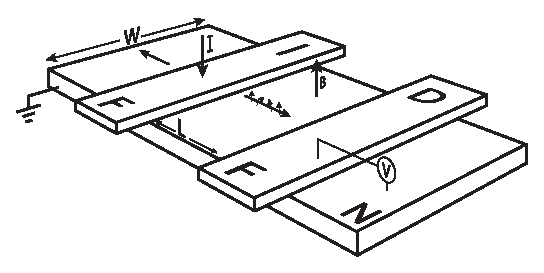
\includegraphics[width=\textwidth]{figures/device}
  \caption{%
    Isometric representation of a nonlocal spin valve in a magnetic field.
    Current is injected into the semiconductor
    through the left ferromagnetic contact.
    The strength of the diffusive spin signal is measured as a voltage
    at the right ferromagnetic contact.
  }\label{fig:spin-device}
\end{figure}

Another excellent candidate for spintronic devices,
TMDs are materials with strong spin-orbit coupling that break spin degeneracy
and provide an intrinsic means to control the spin signal.
In particular, TMDs show a strong coupling
between polarized light and their valley degree of freedom.
Since each band is spin-split, controlled optical excitations
may selectively activate carriers of a single valley and spin population.
Additionally, each valley has opposite Berry curvature, so
electrons in different valleys drift in opposite directions transverse
to an applied in-plane electric field.

\Cref{s:dichalcogenides} of this thesis
characterizes the possible superconducting phases for monolayer TMDs
in a regime where the spin and valley degrees of freedom are locked.
We consider phases arising from proximity to a normal superconductor
or effective attractive electron-electron interactions.
The valley selective optical excitation rules
and topological character are reproduced
in the context of the superconducting state.

\begin{figure}
  \centering
  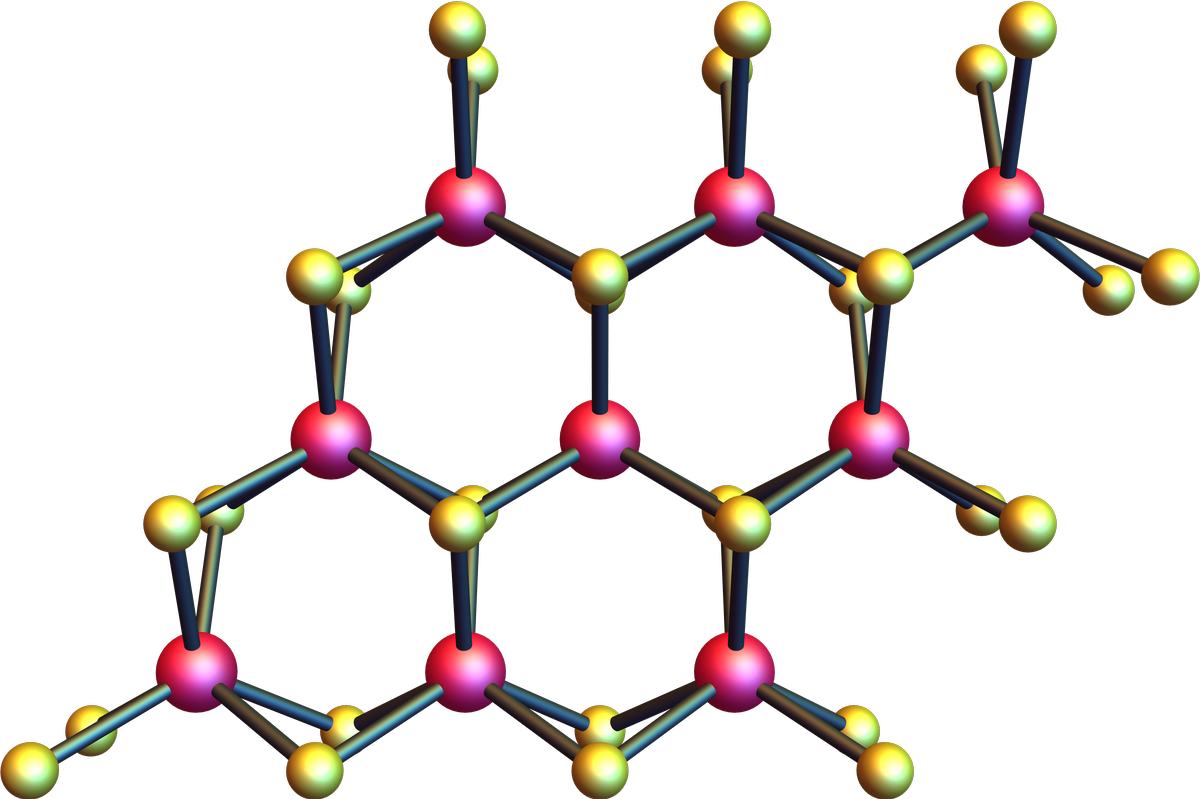
\includegraphics[width=0.7\textwidth]{figures/tmd-crystal-top.png}
  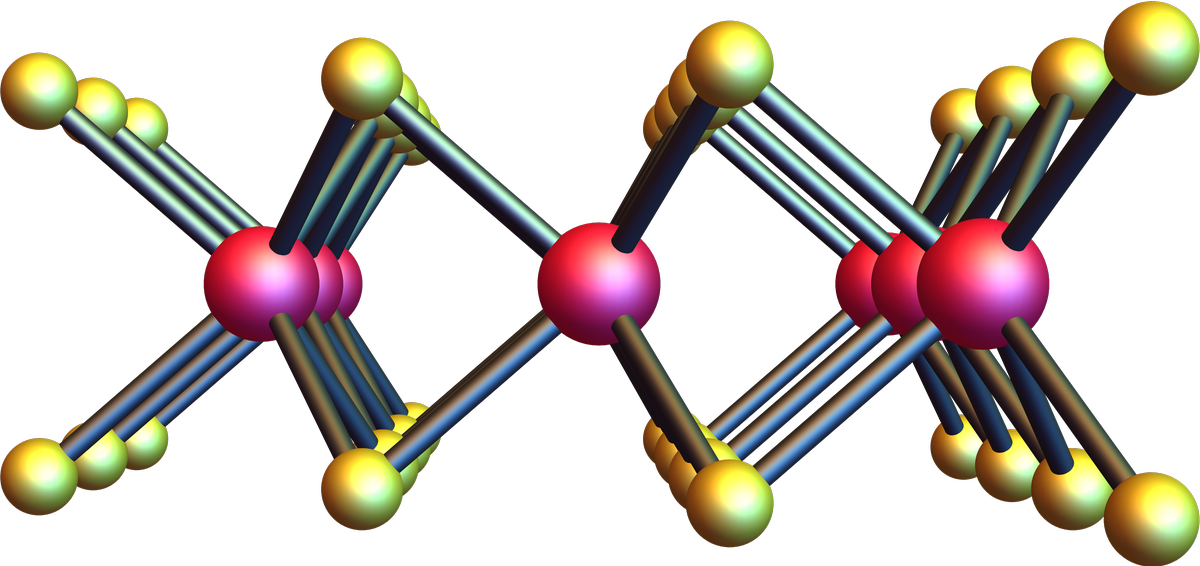
\includegraphics[width=0.7\textwidth]{figures/tmd-crystal-side.png}
  \caption{%
    Top and side views of the crystal structure of monolayer \ce{MoS2}.
  }\label{fig:tmd-crystal}
\end{figure}


  \chapter{Spin Lifetime}
  \section{Introduction}

Spintronic devices rely on the ability to
inject, transport, manipulate, and detect spins
\cite{%
  Wolf16112001,%
  RevModPhys.76.323%
}.
The typical architecture involves ferromagnetic electrodes
deposited on a conducting medium
\cite{%
  1990ApPhL..56..665D,%
  Jedema2001%
}.
Driving a current across the junction of a magnetic element
and a nonmagnetic metal leads to spin injection (also called spin accumulation)
\cite{%
  PhysRevLett.55.1790,%
  Jedema2001,%
  Yang2008,%
  PhysRevLett.94.196601%
}.
The injected spins either diffuse in nonlocal spin valve geometry,
or are driven by applied fields across the conducting channel.
The former has the advantage that the observed spin signal
is not corrupted by accompanying charge current.
During this transit, scattering processes dephase the spins
and thus degrade the chemical potential imbalance
between spins of opposite orientation.
The residual difference is detected by a ferromagnetic electrode
whose magnetization can be flipped by applying external fields.

The performance of devices is determined by a number of parameters
associated with the basic processes described above.
The efficiency of spin injection, the diffusion length
(or equivalently the diffusion constant and spin relaxation time),
the distance between the injector and detector,
and resistivities of various components such as the electrodes,
the junction, and the conducting channel,
are some of the ingredients that contribute to the measured magnetoresistance.
As such, having good injection efficiency coupled with long spin lifetimes
is crucial for the viability of spintronic applications.
The discovery of graphene
\cite{Novoselov22102004}
has been of particular interest in this regard
because of its tunable conductivity, high mobility, and low spin-orbit coupling.
Moreover, the two dimensional nature allows
for efficient device design and spin manipulation.
Theoretical estimates for spin lifetimes of a few microseconds
\cite{%
  PhysRevB.74.155426,%
  Trauzettel2007%
}
are leading to a concerted effort in realizing
spin based transistors and spin valves
\cite{%
  Tombros2007,%
  JJAP.46.L605,%
  Cho2007,%
  PhysRevLett.101.046601,%
  1704408,%
  Han2012,%
  Han2012369,%
  PhysRevB.80.241403%
}.

Unfortunately, the best measured spin lifetimes
via the Hanle spin precession technique are in the
\SIrange{50}{200}{\pico \second} range
\cite{%
  PhysRevB.80.241403,%
  Tombros2007,%
  PhysRevB.80.214427,%
  PhysRevLett.104.187201%
}.
The large discrepancy is yet to be explained.
The linear scaling of spin and transport lifetimes
\cite{PhysRevB.80.241403}
suggested that the dominant scattering mechanism in the conducting channeling
is of the Elliot-Yafet
\cite{PhysRev.96.266}
type.
Surprisingly, in the regime of small spin lifetimes
($∼ \SI{100}{\pico \second}$),
Coulomb scattering was shown not to be the dominant mechanism
\cite{PhysRevLett.104.187201}.
The more important determining factor of the lifetime
was found to be the nature of the interface between
the magnetic electrode and the conducting channel.
Tunneling contacts suppress spin relaxation, and lifetimes of
\SI{771}{\pico \second}
were reported at room temperature, increasing to
\SI{1.2}{\nano \second} at \SI{4}{\kelvin}
\cite{PhysRevLett.107.047207}.
On the other hand, low resistance barriers lead to considerable
uncertainty in the determination of the lifetimes.

Over the last few years, characterizing the nature of the spin dynamics
at the interface has garnered much attention.
A key contribution in this effort is the generalization
of the standard theoretical approach
of calculating the nonlocal magnetoresistance
with and without the magnetic field.
Recent efforts study the effect of including the contact resistance
\cite{%
  PhysRevB.80.214427,%
  PhysRevB.67.052409%
},
and alternatively relaxing the normally infinite boundary conditions
in favor of a finite channel size
\cite{1404.6276v1}.
The approach relies on numerically solving the Bloch equation
to generate Hanle precession curves and then fitting observed data.

In this paper, we present the closed form expression
for the precession curves with finite contact resistance,
and analytically discuss the various parameters regimes
that show qualitatively different behaviors.
The fits to data reproduce the results in the literature
and provide a means to understand the effect of the contacts
which were previously obtained by numerical simulations.

The paper is organized as follows.
In \cref{s:model} we provide the basic model, define the relevant parameters,
and present an expression for the nonlocal resistance $\rNL$.
The primary result is given by \cref{eq:f}.
In \cref{s:fits} the solution for $\rNL$ is fitted to data.
In \cref{s:regimes} we analyze the various regimes which are determined by
the diffusion length, length of the device, and the contact resistance.
\Cref{s:summary} ends with a summary of the results and future directions.

  \section{Model}
\label{s:model}

\begin{figure}
  \caption{
    The geometry of the nonlocal spin valve analyzed in this paper is shown.
    There are two ferromagnetic electrodes placed on a conducting channel.
    Current $I$ flows into the left electrode,
    while the potential $V$ is measured at the right electrode.
    The nonlocal resistance is defined as the ratio $V / I$.
    For spin dependent phenomena, the relevant quantity of interest
    is the difference between the nonlocal resistance for the parallel
    and antiparallel orientations of magnetization of the two electrodes.
  }
  \label{fig:nonlocal_spin_valve}
  \input{components/tikz-nonlocal_spin_valve/tex/_head}
  \begin{tikzpicture}[scale=0.7]
    \input{components/tikz-nonlocal_spin_valve/tex/_nonlocal_spin_valve}
  \end{tikzpicture}
\end{figure}

The assumed device geometry is shown in \cref{fig:nonlocal_spin_valve}.
Two ferromagnetic contacts ($F$) are deposited
on the normal semiconductor ($N$).
A spin-polarized current $I$ is injected through the contact at $x = 0$
and flows in the $x ≤ 0$ region of the semiconductor.
The voltage difference $V$ is measured at
$x = L$ between the contact and the semiconductor.
The nonlocal resistance is $\rNL = V / I$
\cite{PhysRevB.67.052409}.

Spin transport is modeled by identifying two spin channels
and their associated three-component spin electrochemical potentials $μ_{↑↓}$.
The majority channel is labeled as up,
while the minority channel is labeled as down.
The voltage difference is proportional to the spin accumulation
$μ_s = \left( μ_↑ - μ_↓ \right) / 2$ at $x = L$.
The spin accumulation in the semiconductor
is assumed to satisfy the steady-state Bloch diffusion equation
\begin{equation}
  D ∇^2 μ_s^N - \frac{μ_s^N}{τ} + ω × μ_s^N = 0 .
\end{equation}
The key parameters are
the contact spacing $L$,
the diffusion constant $D$,
the spin lifetime $τ$,
the spin diffusion length $λ = \sqrt{D τ}$,
and $ω = \left( g μ_B / ℏ \right) B$ which is proportional to
the applied magnetic field $B$ and the gyromagnetic ratio $g = 2$.

For contacts which cover the width of the channel,
the transport is uniform along $y$.
Since the channel is two-dimensional, $μ_s^N$ will only vary along $x$.
We enforce the boundary condition $μ_s^N → 0$ at $x → ± ∞$
and the continuity of the current and spin current.
A detailed derivation is given in \cref{s:appendix} and reveals
\begin{equation}
  \label{eq:nonlocal_resistance}
  \rNL^± = ± p_1 p_2 R_N f .
\end{equation}
The overall sign corresponds to
parallel and antiparallel ferromagnetic alignments.
Specifically, we find a resistance scale
\begin{equation}
  R_N = \frac{λ}{W L} \frac{1}{σ^N} ,
\end{equation}
and the function
\begin{multline}
  \label{eq:f}
  f = \re \left( \left\{
        \vphantom{
          \frac{
            \sinh{ \left[ \left( L / λ \right) \sqrt{1 + i ω τ} \right] }
          }{\sqrt{1 + i ω τ}}
        }
        2 \left[ \sqrt{1 + i ω τ} + \frac{λ}{2} \left( \frac{1}{r_0} + \frac{1}{r_L} \right) \right]
        e^{\left( L / λ \right) \sqrt{1 + i ω τ}}
        \right. \right. \\ \left. \left.
        + \frac{λ^2}{r_0 r_L} \frac{
            \sinh{ \left[ \left( L / λ \right) \sqrt{1 + i ω τ} \right] }
          }{\sqrt{1 + i ω τ}}
      \right\}^{-1} \right) .
\end{multline}

Note that $f$ is unitless and depends only on the scales
$L / λ$, $ω τ$, and $λ / r_i$.
The parameters $r_i$ with $i$ either $0$ for
the left contact or $L$ for the right are
\begin{equation}
  \label{eq:r-parameter}
  r_i = \frac{R_F + R_C^i}{\rSQ} W ,
\end{equation}
where $R_F$ is the resistance of the ferromagnet
and $R_C^i$ are the individual contact resistances,
$W$ is the graphene flake width, and
\begin{equation}
  \label{eq:square_resistance}
  \rSQ = W / σ^N ,
\end{equation}
is the graphene square (sheet) resistance
given in terms of the semiconductor conductivity $σ^N$.
The resistances $R_F$ and $R_C^i$ are the effective resistances
of a unit cross sectional area.
They are defined in \cref{eq:contact.resistance,eq:ferromagnet.resistance}.
To obtain an expression in terms of the ohmic resistances,
one must make the substitutions
$R_F → W_F W R_F$ and $R_C^i → W_F W R_C^i$,
where $W_F$ is the contact width, i.e., $W_F W$ is the contact area.
We will use the same symbols for either resistance type
when the meaning is clear.
The polarizations $p_1$ and $p_2$, defined in \cref{eq:polarizations},
model the effective current injection.
They depend on the resistances and the spin polarizations
of the semiconductor and the individual contacts.

The expression $Δ \rNL = \abs{\rNL^+ - \rNL^-}$
measures the difference in signal between
parallel and antiparallel field alignments.
We combine $P^2 = \abs{p_1 p_2}$
\footnote{
  Assuming the polarizations $P_σ^F$ and $P_Σ^L$
  have the same sign bounds $P ≤ 1$.
},
and write
\begin{equation}
  \label{eq:nonlocal_resistance.difference}
  Δ \rNL = 2 P^2 R_N \abs{f} ,
\end{equation}
with
\begin{equation}
  R_N = \frac{λ}{W} \frac{1}{σ_G} ,
\end{equation}
where $σ_G = σ^N L$ is the graphene conductance normally given in units of
$\si{\milli \siemens} = \left( \si{\milli \ohm} \right)^{-1}$.

  \section{Fits}
\label{s:fits}

Data presented in figure 4 from \cite{PhysRevLett.105.167202}
was fit to the model presented here.
Fits done using Python and matplotlib \cite{Hunter:2007}.
Links to the source code along with instructions
on how to create similar fits and figures are available online
\footnote{
  An online portal with links to the code used to prepare this work is located at
  \href{http://evansosenko.com/spin-lifetime/}{evansosenko.com/spin-lifetime/}.
}.

We assume similar contacts, $R_C = R_C^0 = R_C^L$.
The resistance of the ferromagnet \ce{Co} is computed as
$R_F = ρ_F λ_F / A_J$,
where $ρ_F$ is the \ce{Co} resistivity,
$λ_F$ is the spin diffusion length of \ce{Co},
and $A_J$ is the junction area estimated at $A_J = W d$,
with $d$ between \SIrange[range-phrase={ and }]{0.5}{50}{\nano \meter}
\cite{PhysRevLett.105.167202}.
Hanle fits were done using a simple least squares algorithm
with nonnegative parameters $τ$, $D$, $R_C$, and $P$.
The polarization $P$ was constrained between zero and one.

\begin{figure}
  \caption{
    Data in figure 4 from \cite{PhysRevLett.105.167202}
    fit to \cref{eq:nonlocal_resistance.difference}
    or \cref{eq:nonlocal_resistance}
    with the following values: \plotFitsInfo.
    The contact type (tunneling, pinhole, or transparent)
    and the contact separation $L$ varies.
  }
  \label{fig:nonlocal_resistance.fits}
  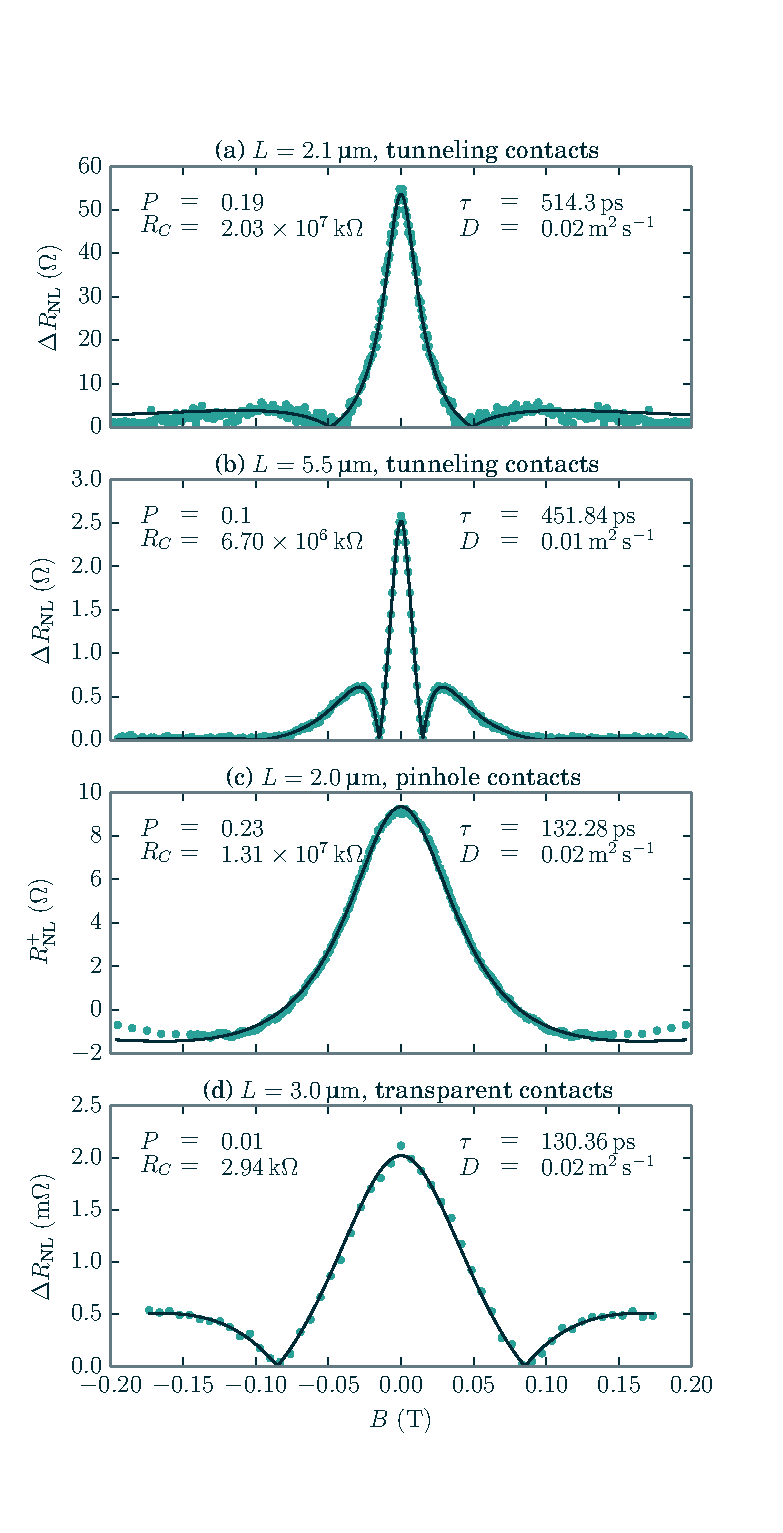
\includegraphics[width=\columnwidth]{figures/plot_fits}
\end{figure}

\Cref{fig:nonlocal_resistance.fits} shows fits of
$Δ \rNL$ given by \cref{eq:nonlocal_resistance.difference}
for devices with tunneling and transparent contacts,
and $\rNL^+$ given by \cref{eq:nonlocal_resistance}
for a device with pinhole contacts
\footnote{
  Parallel and antiparallel data for this device was only available
  at dissimilar field values, thus $Δ \rNL$ could not be fit.
}.
Fits (a), (b), and (c) with tunneling and pinhole contacts give large
$R_C ∼ \SI{e7}{\kilo \ohm}$ and lifetimes equivalent to fitting with $R_C → ∞$,
while (d) with transparent contacts gives a reduced $R_C ∼ \SI{3}{\kilo \ohm}$
and a lifetime increased by at most a factor of two
(compare to \SI{78}{\pico \second} for $R_C → ∞$).
For tunneling contacts, the polarization $P$ is \SIrange{25}{60}{\percent}
smaller than the lower bound given in \cite{PhysRevLett.105.167202},
while for transparent contacts, $P$ is reduced by an order of magnitude.

Note that we have used $R_C$ as a fitting parameter.
In most devices, this quantity can be experimentally determined,
thus further constraining the fitting algorithm.
As we will discuss further in the next section, a fact that becomes apparent
from our analytic result is that the relevant scale is $λ / r$.
Once $r$ becomes larger than $λ$,
all of the corrections to the $R_C → ∞$ limit Hanle curves become very small.
In other words, once $r ≫ λ$,
the fit is insensitive to the actual value of the contact resistance.
The fact that we quote a resistance of order \SI{e7}{\kilo \ohm} in fits (a), (b), and (c)
in \cref{fig:nonlocal_resistance.fits}
results from the built-in accuracy we demand of the fitting algorithm.
A good fit can be obtained for any $r$ as long as it is larger than $λ$.

  \section{Regimes}
\label{s:regimes}

In this section we discuss the various limits of
the expression describing the Hanle precession curve.
First, we show that the commonly used results for zero magnetic field
and tunneling contacts are correctly reproduced.
Next, we discuss regimes where
appropriate scaling will give non-unique Hanle fits.
In the following, we consider the case $r = r_0 = r_L$ of similar contacts.

In the limit of tunneling contacts, $R_C^0, R_C^L ≫ R_F$.
Putting $r_0, r_L → ∞$ gives $p_1 p_2 → \left( P_Σ^L \right)^2$ and
\begin{equation}
  f^∞ = \re{\frac{e^{- \left( L / λ \right) \sqrt{1 + i ω τ}}}{2 \sqrt{1 + i ω τ}}} ,
\end{equation}
which is of the same form as found in appendix B of
\cite{PhysRevB.37.5312}
(we will denote this limit with the superscript $∞$).
Fitting with this expression was found to give results equivalent
to fitting with the Hanle equation
\begin{equation}
  \label{eq:hanle_integral}
  \rNL^± = ± \sNL ∫_0^∞ \frac{e^{-t / τ}}{\sqrt{4 π D t}}
             \exp{\left[- \frac{L^2}{4 D t} \right]} \cos{ω t} \: dt .
\end{equation}
The agreement is expected as an explicit integration of \cref{eq:hanle_integral}
yields the same analytic expression with the identification
$\sNL = {p_1 p_2 D} / {W σ_G}$.
In the additional limit of zero magnetic field,
\begin{equation}
  Δ \rNL = \left( P_Σ^L \right)^2 R_N e^{- L / λ} ,
\end{equation}
which agrees with equation (6) in
\cite{PhysRevB.67.052409}.

Let $f_0$ denote $f$ at zero magnetic field,
\begin{equation}
  f_0 = \left[ 2 \left( 1 + λ / r \right) e^{L / λ} + \left( λ / r \right)^2 \sinh{L / λ} \right]^{-1} ,
\end{equation}
which agrees with equation (3) in
\cite{PhysRevB.80.214427}.

To further explore the nature of the Hanle curves,
we exploit the fact that it only depends on
the dimensionless ratios $λ / r$, $L / λ$, and $ω τ$.
The only other parameter of the conducting channel that enters the expression
is the overall scale $λ$ in $R_N$.
The expression $f$ contains three terms
which are of zeroth, first, and second order in $λ / r$.
Thus, as the contact resistance decreases,
one goes from a device dominated by the first term to one dominated by the last.
But precisely how this comes about depends on the value of $ω τ$.

For infinite contact resistance, it was pointed out that any rescaling
of $g$, $τ$ and $D$ that leaves $λ$ and $ω τ$ unchanged
leads to the same Hanle precession curves
\cite{Swartz2013}.
Our result shows that the same is also true
when the contact resistance is taken into account.
In numerical simulations, interesting features were observed
when $L / λ ≪ 1$ and $r / λ ≪ 1$
\cite{PhysRevB.86.235408}.

To compare across regimes,
we first normalize the data to its value at zero magnetic field.
In devices where $λ / r ≫ 1$, the normalization factor is
\begin{equation}
  f_0 = \frac{2 e^{- L / λ}}{\left( λ / r \right)^2} .
\end{equation}
In this regime, if $D$ is not very different
from the infinite contact resistance value,
then the lifetime can be large, i.e., $τ ≫ \SI{1}{\nano \second}$.
As one tunes the magnetic field $\sqrt{ω τ} ≫ 1$, for small values of the field,
and for much of the curve, we can approximate $1 + i ω τ ≈ i ω τ$.
An interesting consequence of this
is that the zero of the Hanle precession curve
becomes independent of the scattering time.
Note that the product
\begin{equation}
   \frac{L}{λ} \sqrt{ω τ} = L \sqrt{\frac{D}{ω}} ,
\end{equation}
which appears in the exponential and oscillating factors below,
is independent of the lifetime.
As one further tunes the magnetic field, the Hanle curve is given by
\begin{equation}
  \label{eq:regime.1.f}
  f = \frac{\sqrt{ω τ}}{\left( λ / r \right)^2}
      e^{- \left( L / λ \right) \sqrt{ω τ / 2}}
      \sin{\left[ \frac{L}{λ} \sqrt{\frac{ω τ}{2}} + \frac{π}{4} \right]} ,
\end{equation}
as long as $λ / r ≫ \sqrt{ω τ} ≫ 1$.
In this limit, the nonlocal resistance scales as
\begin{equation}
  \label{eq:regime.1.nonlocal_resistance}
  Δ \rNL ∝ \frac{λ \sqrt{ω τ}}{\left( λ / r \right)^2} = r^2 \sqrt{\frac{ω}{D}} ,
\end{equation}
and the normalized nonlocal resistance as
\begin{equation}
  f / f_0 ∝ \sqrt{ω τ} .
\end{equation}

On further increasing the field,
$\sqrt{ω τ} ≫ λ / r ≫ 1$, we get
\begin{equation}
  \label{eq:regime.2.f}
  f = \frac{1}{2 \sqrt{ω τ}}
      e^{- \left( L / λ \right) \sqrt{ω τ / 2}}
      \cos{\left[ \frac{L}{λ} \sqrt{\frac{ω τ}{2}} + \frac{π}{4} \right]} .
\end{equation}
In this limit, the nonlocal resistance scales as
\begin{equation}
  \label{eq:regime.2.nonlocal_resistance}
  Δ \rNL ∝ \frac{λ}{\sqrt{ω τ}} = \sqrt{\frac{D}{ω}} ,
\end{equation}
and the normalized nonlocal resistance as
\begin{equation}
  \label{eq:regime.2.ratio}
  f / f_0 ∝ \frac{\left( λ / r \right)^2}{\sqrt{ω τ}} = D \sqrt{\frac{τ}{ω r^4}} .
\end{equation}

In the limits of \cref{eq:regime.1.f,eq:regime.2.f},
the zeros of the Hanle fit are independent of the lifetime
and are determined by $D$ though the condition
\begin{equation}
  L \sqrt{\frac{D}{2 ω}} + \frac{π}{4} = \frac{n π}{2} ,
\end{equation}
where $n = 0$ for \cref{eq:regime.1.f} and $n = 1$ for \cref{eq:regime.2.f}.

\begin{figure}
  \centering
  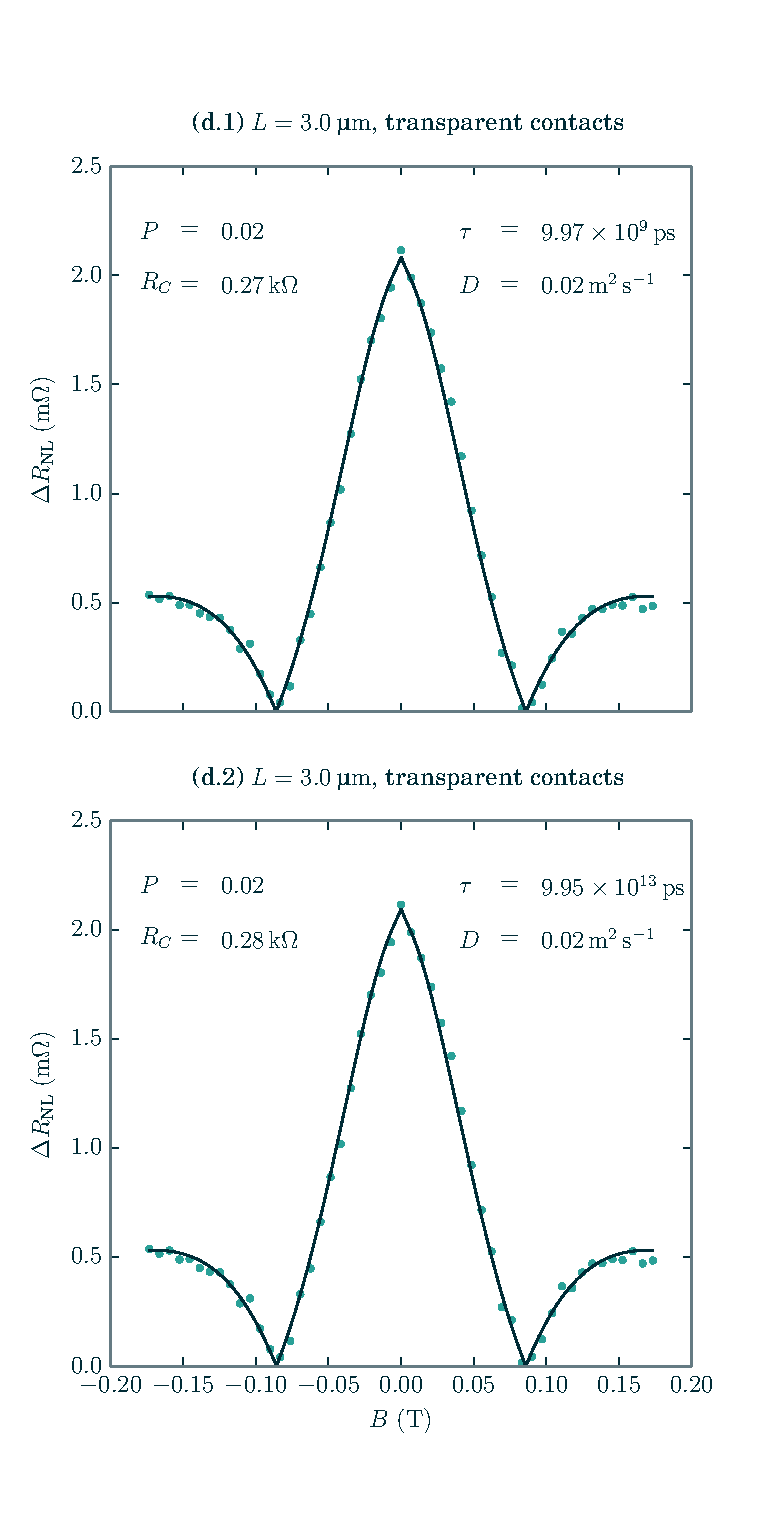
\includegraphics[height=0.8\textheight]{figures/plot_fits_large_lifetime}
  \caption{%
    Data in figure 4 (d) from~\cite{PhysRevLett.105.167202}
    fit to \cref{eq:nonlocal_resistance}
    with the same values as in
    \cref{fig:nonlocal_resistance.fits} (d).
    Fits with lifetimes that differ by four orders of magnitude
    were obtained by using different starting values for $τ$.
    These fits are otherwise similar with the exception of the lifetime,
    demonstrating the $τ$-independent scaling in
    \cref{eq:regime.1.nonlocal_resistance}.
    The $χ^2$ for \cref{fig:nonlocal_resistance.fits} (d)
    is \SI{2}{\percent} less than the $χ^2$ for
    \cref{fig:nonlocal_resistance.large_lifetime}.
  }\label{fig:nonlocal_resistance.large_lifetime}
\end{figure}

Note that fitting is insensitive to $τ$ in the limit of
\cref{eq:regime.1.nonlocal_resistance}
or \cref{eq:regime.2.nonlocal_resistance}.
As an example of this,
\cref{fig:nonlocal_resistance.large_lifetime} shows nearly identical fits
with lifetimes that differ by four orders of magnitude.
These fits were obtained by choosing large starting values for $τ$.
For \cref{fig:nonlocal_resistance.fits} (d)
and \cref{fig:nonlocal_resistance.large_lifetime},
$χ^2 ∼ \SI{7e-8}{}$, but the $χ^2$ for
\cref{fig:nonlocal_resistance.fits} (d)
is \SI{2}{\percent} less than the $χ^2$ for
\cref{fig:nonlocal_resistance.large_lifetime}.
In \cref{fig:nonlocal_resistance.fits} (d),
$λ / r ≫ \sqrt{ω τ}$ and $ω τ ∼ 1$ for most of the curve,
so the approximation $1 + i ω τ ≈ i ω τ$ does not hold.
However, \cref{fig:nonlocal_resistance.large_lifetime}
is in the limit of \cref{eq:regime.1.nonlocal_resistance}
for all points (save the origin).
Thus, in limit of small $r$, the fitted value of $τ$ is unreliable
unless one carefully controls the fitting procedure.

The evolution of the expression for the Hanle curve
is an interesting insight into the behavior of the device.
Fitting data on devices with small contact resistances
with the functional form applicable to infinite contact resistance
yields unreliable parameters.
In particular, they were numerically shown
to severely underestimate the spin lifetime
\cite{PhysRevB.86.235408}.

Further analytic progress can be made if one assumes that
lifetimes as estimated with infinite contact resistance are long
enough that the approximation of $\sqrt{ω τ} ≫ λ / r ≫ 1$
is still valid for much of the data being analyzed.
For this case, at infinite contact resistance,
the normalized nonlocal resistance is given by
\begin{equation}
  \frac{f^∞}{f^∞_0} = \frac{1}{ \sqrt{ω τ}}
                      e^{- \left( L / λ \right) \sqrt{ω τ / 2}}
                      \cos{\left[ \frac{L}{λ} \sqrt{\frac{ω τ}{2}} + \frac{π}{4} \right]} .
\end{equation}
Provided $D$ remains constant,
this will yield the same curve with finite contact resistance if
\begin{equation}
  \label{eq:lifetime_scale.infinity}
  \frac{1}{τ^∞} = D^2 \frac{τ}{r^4} .
\end{equation}
In other words, if we fix $τ$ and ask what happens to the fitted value
assuming infinite contact resistance as a function of decreasing $r$,
\cref{eq:lifetime_scale.infinity} shows that it will decrease as well.
For $D$ fixed, $τ^∞ ∝ r^4$.
While the general trend is consistent with
\cite{PhysRevB.86.235408},
the quantitative agreement is limited by
the approximations made for analytic convenience.

  \section{Summary}
\label{s:summary}

In this paper we have analyzed the effect of contact resistance
on spin lifetimes determined via the Hanle spin prescession technique in nonlocal spin valves.
The general expression for the precession curves given in \cref{eq:f} is the main new result.
While aspects of the discussed phenomena have been addressed numerically before,
an analytic solution is obtained here which allows for detailed characterization of the device.
In particular, general features of scaling as well as various limits and regimes can be analyzed.
In addition, the solution allows for fitting data using standard curve fitting algorithms.

\subsection{Acknowledgments}

We acknowledge useful discussions with Roland Kawakami, Adrian Swartz, and Sung-Po Chao.
The work was partially supported by a UCR Senate Research Grant.

  \section{Appendix}

In this appendix we derive an expression for
the nonlocal resistance for finite contact resistance.
We first present the key definitions and critical boundary conditions.
We then derive the relation between the nonlocal resistance
and the spin chemical potential at the far contact, $μ_s^N (L)$.
Finally, we solve the diffusion equation
inside the semiconductor to find $μ_s^N (L)$.

\subsection{Definitions}

Many of the definitions and results in this section are taken from
\cite{ActaPhysicaSlovaca.57.4_5.565-907}.
The chemical potential and spin chemical potential are defined in terms
of the spin-up and spin-down chemical potentials,
\begin{subequations}\label{eq:potentials}
  \begin{alignat}{2}
    & μ   && = \frac{1}{2} \left( μ_↑ + μ_↓ \right), \\
    & μ_s && = \frac{1}{2} \left( μ_↑ - μ_↓ \right).
  \end{alignat}
\end{subequations}
The material conductances and polarization are defined in terms
of the spin-up and spin-down conductances,
\begin{subequations}\label{eq:conductances}
  \begin{alignat}{2}
    & σ   && = σ_↑ + σ_↓, \\
    & σ_s && = σ_↑ - σ_↓, \\
    %
    \label{eq:material.polarization}
    & P_σ && = \frac{σ_s}{σ}.
  \end{alignat}
\end{subequations}
The gradient of the chemical potentials drives a current and spin current,
\begin{subequations}\label{eq:currents}
  \begin{alignat}{3}
    & J_{↑↓} && = σ_{↑↓} ∇μ_{↑↓}, \\
    %
    \label{eq:currents.current}
    & J      && = J_↑ + J_↓ & = σ   ∇μ + σ_s ∇μ_s, \\
    %
    \label{eq:currents.spincurrent}
    & J_s    && = J_↑ - J_↓ & = σ_s ∇μ + σ   ∇μ_s.
  \end{alignat}
\end{subequations}
To indicate the material, any of the above can have a superscript
$N$ (normal semiconductor) or $F$ (ferromagnet).

The contact conductances and polarization are defined in terms
of the spin-up and spin-down contact conductances,
\begin{subequations}\label{eq:contact_conductances}
  \begin{alignat}{2}
    & Σ   && = Σ_↑ + Σ_↓, \\
    & Σ_s && = Σ_↑ - Σ_↓, \\
    %
    \label{eq:contact.polarization}
    & P_Σ && = \frac{Σ_s}{Σ}.
  \end{alignat}
\end{subequations}
The mismatch of the chemical potentials across the contact
drives a current and spin current,
\begin{subequations}\label{eq:contact_currents}
  \begin{alignat}{2}
    & J_{↑↓}^C && = Σ_{↑↓} {\left( μ^N_{↑↓} - μ^F_{↑↓} \right)}_c, \\
    %
    & J^C      && = J_↑^C + J_↓^C, \\
    & J_s^C    && = J_↑^C - J_↓^C.
  \end{alignat}
\end{subequations}
The subscript $c$ will always denote the function evaluated at the contact.

We will use the term current to refer to $J$,
when in fact this is a particle current density.
For constant $J$, the physical charge current $I$ will be related to $J$
by a relation $I = - A J / e$ for some characteristic area $A$.

To reduce the number of subscripts and superscripts in the following,
we adopt the notation for the potentials
\begin{subequations}
  \begin{equation}
    \begin{aligned}
    & \begin{alignedat}{2}
        & u && = μ^N_s, \\
        & v && = μ^N,
      \end{alignedat}
    & \begin{alignedat}{2}
        & φ && = μ^F_s, \\
        & ψ && = μ^F,
      \end{alignedat}
    \end{aligned}
  \end{equation}
  and currents
  \begin{equation}
    \begin{alignedat}{2}
      & ȷ   && = J_s, \\
      & J_c && = J^C, \\
      & ȷ_c && = J_s^C.
    \end{alignedat}
  \end{equation}
\end{subequations}

We rewrite \cref{eq:contact_currents} as
\begin{subequations}\label{eq:contact_currents.2}
  \begin{alignat}{3}
    \label{eq:contact_currents.2.current}
    & J_c && = Σ   \left( v_c - ψ_c \right) && + Σ_s \left( u_c - φ_c \right),
    \\
    \label{eq:contact_currents.2.spincurrent}
    & ȷ_c && = Σ_s \left( v_c - ψ_c \right) && + Σ   \left( u_c - φ_c \right),
  \end{alignat}
\end{subequations}
and \cref{eq:conductances,eq:currents} as
\begin{equation}
  \label{eq:bdry_current}
  ȷ = P_σ J + 4 \frac{σ_↑ σ_↓}{σ} ∇μ_s.
\end{equation}

Using \cref{eq:contact_conductances,eq:contact_currents.2},
\begin{equation}
  \label{eq:bdry_current_contact}
  ȷ_c = P_Σ^i J_c + {R_C^i}^{-1} \left( u_c - φ_c \right),
\end{equation}
where the contact resistance is
\begin{equation}
  \label{eq:contact.resistance}
  R_C^i = \frac{Σ^i}{4 Σ_↑^i Σ_↓^i}.
\end{equation}
The superscript $i$ allows for contacts with difference conductances.

\subsection{Boundary conditions}

In this sections, we derive the relations between
the potentials and the currents
This corresponds to the needed boundary conditions.

\subsubsection{Semiconductor}

For the semiconductor, $σ^N_↑ = σ^N_↓ = σ^N / 2$, so $P_σ^N = 0$.
Evaluating \cref{eq:bdry_current} at the contact gives
\begin{equation}
  \label{eq:bdry_current.semiconductor}
  ȷ^N_c = σ^N {( ∇u )}_c.
\end{equation}

\subsubsection{Ferromagnet}

For the ferromagnet, one assumes $μ_s^F$ satisfies
the one dimensional diffusion equation.
We choose the $z'$ coordinate antiparallel to $z$ with origin at the contact.
The equation
\begin{equation}
  \label{eq:diffusion.ferromagnet}
  φ'' \left( z' \right) - k_F^2 φ \left( z' \right) = 0,
\end{equation}
with the boundary condition
$\lim_{z' → - ∞} φ(z') = 0$
has solution
\begin{equation}
  \label{eq:diffusion.ferromagnet.solution}
  φ(z') = φ_c e^{k_F z'} ,
\end{equation}
where $φ_c = φ(0)$ is a yet undetermined constant.
Putting this into \cref{eq:bdry_current} and evaluating it at the contact gives
\begin{equation}
  \label{eq:bdry_current.ferromagnet}
  ȷ^F_c = P_σ^F J^F_c + R_F^{-1} φ_c,
\end{equation}
where the ferromagnet resistance is
\begin{equation}
  \label{eq:ferromagnet.resistance}
  R_F = \frac{σ^F}{4 σ_↑^F σ_↓^F k_F}.
\end{equation}
Here, $λ_F = 1 / k_F$ is the spin diffusion length in the ferromagnet.

\subsubsection{Continuity assumptions}

At the contact, the current and spin current are assumed continuous,
\begin{subequations}\label{eq:continuity.current}
  \begin{alignat}{3}
    & J_c && = J^F_c && = J^N_c, \\
    & ȷ_c && = ȷ^F_c && = ȷ^N_c.
  \end{alignat}
\end{subequations}
Using
\cref{eq:bdry_current.ferromagnet,eq:bdry_current_contact,eq:continuity.current}
we find the relation
\begin{subequations}\label{eq:bdry_solutions}
  \begin{equation}
    \label{eq:bdry_solutions.current}
    \left( P_σ^F R_F + P_Σ^i R_C^i \right) J_c
    = \left( R_F + R_C^i \right) ȷ_c - u_c,
  \end{equation}
  and that $φ_c$ is determined by
  \begin{equation}
    \label{eq:bdry_solutions.potential}
    R_F^{-1} φ_c
    = \frac{\left( P_Σ^i - P_σ^F \right) R_C^i ȷ_c + P_σ^F u_c}
           {P_σ^F R_F + P_Σ^i R_C^i}.
  \end{equation}
\end{subequations}
In the special case of zero current at the contact ($J_c = 0$),
\cref{eq:bdry_solutions} reduces to
\begin{subequations}\label{eq:bdry_solutions.zero}
  \begin{alignat}{2}
    \label{eq:bdry_solutions.zero.current}
    & ȷ_c && = \frac{1}{R_F + R_C^i} u_c,
    \\
    \label{eq:bdry_solutions.zero.potential}
    & φ_c && = \frac{R_F}{R_F + R_C^i} u_c.
  \end{alignat}
\end{subequations}

\subsection{Nonlocal resistance}
\label{s:appendix:nonlocal_resistance}

In this section we derive the precise relation between $\rNL$ and $μ_s^N (L)$.
Note that we may write in general, for some $\bar{μ}$,
\begin{equation}
  μ = \bar{μ} + P_σ μ_s ,
\end{equation}
and, following
\cite{PhysRevB.67.052409},
define the voltage due to the difference
in the chemical potentials across the contacts by
\begin{equation}
  V_c = \left( \bar{μ}_c^N - \bar{μ}_c^F \right) / e.
\end{equation}

We assume a fixed current $J_0 = \abs{J_0} > 0$
flows down through the contact at $x = 0$
and to the left in the semiconductor for $x ≤ 0$,
and no current flows for $x > 0$.
The experimentally measured quantity is the
nonlocal resistance $\rNL = V_L / I_0$,
where $I_0 = - W L J_0 / e$ is the current through the contact at $x = 0$.
It is convenient to introduce the effective nonlocal resistance $\rNLeff$
defined by
\begin{equation}
  \rNLeff = W L \rNL = - e V_L / J_0 = \frac{\bar{μ}_c^F - \bar{μ}_c^N}{J_0}.
\end{equation}
To determine $\rNL$, we must express the difference
of these chemical potentials in terms of $μ_s^N (L)$.

Since there are two ferromagnetic contacts,
we have separate functions $ψ$ and $φ$ for each contact
which we will denote by $ψ^0$, $φ^0$, and $ψ^L$, $φ^L$.
From \cref{eq:diffusion.ferromagnet.solution}, we have
\begin{subequations}
  \begin{align}
    φ^0 \left( z' \right) & = φ_0 e^{k_F z'}, \\
    φ^L \left( z' \right) & = φ_L e^{k_F z'}.
  \end{align}
\end{subequations}

The physical restriction on the current flow in the semiconductor
is imposed by noting that since $σ_s^N = 0$,
\cref{eq:currents.current} gives $J^N = σ^N ∇v$, so we must have
\begin{equation}
  v_x (x) =
    \begin{cases}
      v_x (0) - \left( J_0 / σ^N \right) x & \text{~for~} x ≤ 0, \\
      v_x (0)                              & \text{~for~} x > 0,
    \end{cases}
\end{equation}
$v_y (x) = v_y (0)$, and $v_z (x) = v_z (0)$.

Using \cref{eq:currents.current},
the restriction on the current flow in each ferromagnet gives
\begin{subequations}
  \begin{align}
    ∇ψ^0 & = \left( J_0 / σ^F \right) - P_σ^F ∇φ^0, \\
    ∇ψ^L & = - P_σ^F ∇φ^L.
  \end{align}
\end{subequations}
Integrating and enforcing
$e V_c = v_x (0) - \left( ψ_c - P_σ^F φ_c \right)$,
\begin{subequations}
  \begin{align}
    & \begin{aligned}
        ψ^0 \left( z' \right) & = - e V_0 + P_σ^F φ_0 \left( 2 - e^{k_F z'} \right) \\
                              & \qquad + v_x (0) + \left( J_0 / σ^F \right) z',
      \end{aligned} \\
    & \begin{aligned}
        ψ^L \left( z' \right) & = - e V_L + P_σ^F φ_L \left( 2 - e^{k_F z'} \right) \\
                              & \qquad + v_x (0).
      \end{aligned}
  \end{align}
\end{subequations}

There is no current at the contact at $x = 0$,
thus \cref{eq:contact_currents.2.current} gives
\begin{equation}
  ψ_L - v_L = P_Σ^L \left( u_L - φ_L \right),
\end{equation}
and with
\cref{eq:bdry_solutions.zero.potential},
we find
\begin{equation}
  \label{eq:rnl.full}
  \rNLeff = \left( ψ_L - v_L \right) - P_σ^F φ_L
          = \left[ P_Σ^L \left( 1 - \frac{R_F}{R_F + R_C^L} \right) - \frac{P_σ^F R_F}{R_F + R_C^L} \right] \frac{u_x (L)}{J_0}.
\end{equation}

\subsection{Diffusion equation}

In this section we show how to solve for $μ_s^N (L)$.
This method is based on the one described in
\cite{PhysRevB.80.214427}.
Inside the semiconductor, $u$ satisfies the diffusion equation
\begin{equation}
  \label{eq:diffusion}
  D ∇^2 u - \frac{u}{τ} + ω × u = 0.
\end{equation}
Here, $D$ is the diffusion constant, $τ$ the spin lifetime,
and $ω = \left( g μ_B / ℏ \right) B$
is proportional to the applied magnetic field
(with $g$ the gyromagnetic ratio and $μ_B$ the Bohr magneton).
The spin diffusion length in the semiconductor is $λ = 1 / k = \sqrt{D τ}$.

The function $u = u(x)$ only varies along $x$,
and we introduce the notation
\begin{equation}
  u_x (x) =
    \begin{cases}
      u_{x-} (x) \text{~for~} x < 0    , \\
      u_{x0} (x) \text{~for~} 0 ≤ x ≤ L, \\
      u_{x+} (x) \text{~for~}     L < x,
    \end{cases}
\end{equation}
with similar expressions for $u_y$ and $u_z$.
The most general solution to \cref{eq:diffusion}
decouples $u_z$ from $u_x$ and $u_y$.
The requirement $\lim_{x → ± ∞} u(x) = 0$ yields
\begin{subequations}
  \begin{alignat}{3}
    & u_{z±} (x) && {}={} && A^∓ e^{∓ k x}, \\
    & u_{z0} (x) && {}={} && A_0^+ e^{k x} {}+{} A_0^- e^{-k x},
  \end{alignat}
\end{subequations}
and
\begin{subequations}
  \begin{alignat}{6}
    & u_{x±} (x) && =   && B^∓ e^{∓ κ x} && {}+{} &&   && C^∓ e^{∓ \bar{κ} x}, \\
    & u_{y±} (x) && = i && B^∓ e^{∓ κ x} && {}-{} && i && C^∓ e^{∓ \bar{κ} x},
  \end{alignat}
  \begin{alignat}{12}
    & u_{x0} (x) && =   && B_0^+ e^{κ x} && {}+{} &&   && B_0^- e^{- κ x} && {}+{} &&   && C_0^+ e^{\bar{κ} x} && {}+{} &&   && C_0^- e^{- \bar{κ} x}, \\
    & u_{y0} (x) && = i && B_0^+ e^{κ x} && {}+{} && i && B_0^- e^{- κ x} && {}-{} && i && C_0^+ e^{\bar{κ} x} && {}-{} && i && C_0^- e^{- \bar{κ} x},
  \end{alignat}
\end{subequations}
where $κ = k \sqrt{1 + i ω τ}$.
The twelve constants $A$, $B$ and $C$
(with their various subscripts and superscripts)
must be determined by imposing the appropriate boundary conditions.

We first require $u$ be continuous at $x = 0$ and $x = L$;
this gives six equations.
We now require a boundary condition on $∇u$,
but $∇u$ cannot be assumed continuous at the contact.
We make the assumption that the total spin current at the contact
is the sum of the spin currents on either side, i.e.,
\begin{subequations}\label{eq:current.sum}
  \begin{alignat}{2}
    & ȷ_0 && = σ^N \left[ - u_-'(0) + u_0'(0) \right], \\
    & ȷ_L && = σ^N \left[ - u_0'(L) + u_+'(L) \right].
  \end{alignat}
\end{subequations}
The signs have been chosen to be consistent with the physical geometry.
The only nonzero component of the current
at the contacts inside the semiconductor
is the $x$ component at $x = 0$, so we use \cref{eq:bdry_solutions.current}.
For all other components there is zero current at the contact, and we use
\cref{eq:bdry_solutions.zero.current}.
Together with \cref{eq:current.sum}, this gives the other six equations,
\begin{subequations}
  \begin{alignat}{8}
    & - & {} & u_{z-}'(0) & {}+{} & u_{z0}'(0) & {}+{} & η_0 u_z(0) && = 0, \\
    &   & {} & u_{z+}'(L) & {}-{} & u_{z0}'(L) & {}+{} & η_L u_z(L) && = 0, \\
    & - & {} & u_{x-}'(0) & {}+{} & u_{x0}'(0) & {}+{} & η_0 u_x(0) && = Δ, \\
    &   & {} & u_{x+}'(L) & {}-{} & u_{x0}'(L) & {}+{} & η_L u_x(L) && = 0, \\
    & - & {} & u_{y-}'(0) & {}+{} & u_{y0}'(0) & {}+{} & η_0 u_y(0) && = 0, \\
    &   & {} & u_{y+}'(L) & {}-{} & u_{y0}'(L) & {}+{} & η_L u_y(L) && = 0,
  \end{alignat}
\end{subequations}
where
\begin{subequations}
  \begin{alignat}{2}
  & η_i^{-1} && = - σ^N \left( R_F + R_C^i \right), \\
  & Δ && = - (- J_0) \left( P_σ^F R_F + P_Σ^0 R_C^0 \right) η_0.
  \end{alignat}
\end{subequations}
We define the $r$-parameter, $r_i = - η_i^{-1}$,
introduced in \cref{eq:r-parameter}.

These equations can be organized
into a matrix equation and solved algebraically.
A solution for $u_z$ corresponds to a condition of vanishing determinant,
\begin{equation}
  e^{-2 L / λ}
  = \left( 1 + \frac{2 r_0}{λ} \right) \left( 1 + \frac{2 r_L}{λ} \right),
\end{equation}
which can never be satisfied%
\footnote{%
  Except at the nonphysical point $L / λ = r_i / λ = 0$.
},
thus $u_z = 0$ is the only allowed solution.
The other two components form an eight dimensional linear system.
Solving this gives the remaining constants, and thus
$u_x (L) = e^{- κ L} B^- + e^{- \bar{κ} L} C^-$.

Finally, by using $p_1 = - σ^N Δ / J_0$ along with \cref{eq:rnl.full},
we can introduce $\rSQ$ from \cref{eq:square_resistance}
and the polarizations
\begin{subequations}\label{eq:polarizations}
  \begin{align}
    p_1 & = \frac{P_σ^F R_F + P_Σ^L R_C^L}{R_F + R_C^L}, \\
    p_2 / p_1 & = \left. \left( 1 - \frac{P_σ^F R_F}{P_Σ^L R_C^L} \right) \middle/
                  \left(1 + \frac{P_σ^F R_F}{P_Σ^L R_C^L} \right) \right. ,
  \end{align}
\end{subequations}
to write
\begin{equation}
  \frac{\rNLeff}{\rSQ}
  = \frac{p_1 p_2}{W / λ} \left[ - \frac{k u_x (L)}{Δ} \right].
\end{equation}
The factor in brackets is the function $f$ given in \cref{eq:f}.


  \chapter{TMD Superconductivity}
  \section{Introduction}

The interplay of spin-orbit interaction and electron-electron interaction
is a fertile area of research where new phases of matter
and novel phenomena have been theoretically conjectured
and experimentally realized
\cite{%
  PhysRevLett.61.2015,%
  PhysRevLett.95.226801,%
  PhysRevLett.96.106802,%
  Konig02112007,%
  RevModPhys.82.3045,%
  RevModPhys.83.1057,%
  doi:10.1146/annurev-conmatphys-020911-125138% chktex 8
}.
Single-layer transition metal group-VI dichalcogenides (TMDs),
\ce{MX2} ($\ce{M} = \ce{Mo}, \ce{W}$
and $\ce{X} = \ce{S}, \ce{Se}, \ce{Te}$),
are direct band gap semiconductors that have all the necessary ingredients
to explore this phenomena
\cite{%
  RadisavljevicB.2011,%
  PhysRevB.84.153402,%
  doi:10.1021/nl2021575,%
  Wang2012,%
  Ye30112012,%
  Bao2013,%
  1.4804936,%
  PhysRevB.88.075409,%
  Xu2014,%
  1508.03068%
}.
While sharing the hexagonal crystal structure of graphene,
they differ in three important aspects:
(1) inversion symmetry is broken, resulting in a gap
as opposed to Dirac nodes;
(2) spin is coupled to momenta, yielding
a large splitting of the valence bands;
and (3) the bands near the chemical potential predominantly have
the transition metal $d$-orbital character
\cite{%
  0022-3719-5-7-007,% chktex 8
  PhysRevB.64.235305,%
  PhysRevLett.105.136805,%
  doi:10.1021/nl903868w,%
  PhysRevB.88.045416,%
  PhysRevB.88.085433%
}.

The nontrivial Berry curvature
associated with the bands near the valleys
is a consequence of strong spin-orbit coupling
enabled by inversion symmetry breaking and heavy elements
such as \ce{Mo} and \ce{W}.
The Berry curvature engenders an effective intrinsic angular momentum
associated with the Bloch wave functions.
Remarkably, spin-preserving optical transitions between valence
and conduction bands are possible,
even though the atomic orbitals involved all have a $d$-character.
Furthermore, the valley-dependent sign of
the Berry curvature leads to selective photoexcitation:
right circular polarization couples to one valley,
and left circular polarization to the other.
Consequently, this enables a number of valleytronic and spintronic applications
that have attracted a lot of attention over the last few years
\cite{%
  RevModPhys.82.1959,%
  PhysRevLett.108.196802,%
  Mak27062014%
}.

We are primarily interested in exploiting
the band structure and valley-contrasting probe afforded by
the nontrivial topology in order to study and manipulate
correlated phenomena in these systems.
In particular, we focus on hole-doped systems,
where an experimentally accessible window in energy
is characterized by two disconnected pieces of
spin non-degenerate Fermi surfaces.
One can preferentially excite electrons from either Fermi surface.
Since the spins are locked to their valley index,
these excitations have specific $s_z$
(where the $z$-axis is perpendicular to the two-dimensional crystal).
We focus on the possible superconducting states and their properties.

Spin-valley locking and its consequence for superconductivity,
dubbed Ising superconductivity, has been previously studied
for heavily doped $p$-type and $n$-type TMDs
\cite{%
  Lu1353,%
  Xi2016,%
  Saito2016,%
  PhysRevB.93.180501,%
  PhysRevLett.113.097001%
},
where Fermi surfaces of each spin are present in each valley.
Our focus is the regime of maximal loss of spin degeneracy where the
effects are most striking
\cite{1604.02134v2}.
The two valleys in the energy landscape generically allow
two classes of superconducting phases:
intervalley pairing with zero center of mass momentum,
and intravalley pairing with finite Cooper pair center of mass.
Since center-of-symmetry is broken and spin degeneracy is lost,
classifications of superconducting states by parity,
i.e., singlet vs.\ triplet, is no longer possible.
In this chapter, we study both extrinsic and intrinsic superconductivity
by projecting the interactions and pairing potential to
the topmost valence band.
We identify the possible phases, and analyze the nature
of the optoelectronic coupling and the response to magnetic fields.
Our main conclusions are as follows:

\introparanum{}
For both proximity to an $s$-wave superconductor,
and due to local attractive density-density interactions,
the leading instability is due to an intervalley paired state,
where the Cooper pair is an equal mixture
of a spin singlet and the $m = 0$ spin triplet.

\introparanum{}
While the valley selectivity of the optical transition is suppressed,
it remains finite.
Consequently, the two quasiparticles
generated by pair-breaking circularly polarized light
are correlated such that one is in the valence band of one valley
and the conduction band of the other.
The valley and bands are determined by the polarity of incident light.

\introparanum{}
The quasiparticles generated in (2)
both have the same charge and Berry curvature.
Thus an anomalous Hall effect is anticipated
as the two travel in the same direction transverse to an applied electric field.

\introparanum{}
An in-plane magnetic field tilts the spin,
modifying the internal structure of the Cooper pair,
however, no pair-breaking is induced in the absence of scalar impurities.
The suppression of the effective interaction leads
to a parametric reduction of the transition temperature.
In the presence of scalar impurities, pair-breaking is enabled,
but the associated critical magnetic field is large.

  \section{Model}

The TMD system is described by
the effective tight-biding, low-energy, two-valley Hamiltonian
\cite{PhysRevLett.108.196802},
\begin{equation}
  \label{eq:tmd:hamiltonian}
  H_τ^0 \ofK
  = a t \left( τ k_x σ_x + k_y σ_y \right) ⊗ I_2
    + \frac{Δ}{2} σ_z ⊗ I_2 - λ τ \left(σ_z - 1 \right) ⊗ S_z.
\end{equation}
The (periodic) Bloch orbital states
(see \cref{s:appendix:tight-binding}) are
\begin{equation}
  \ketOrbitalK{ν}
  = \frac{T_{\vK +  τ \vc{K}}}{\sqrt{N}}
    ∑_{n = 1}^N e^{i \left( \vK + τ \vc{K} \right) ⋅ \vRn{n}}
    T \of{\vRn{n}} \ketOrbital{ν},
\end{equation}
where $N$ is the number of \ce{M}-type atoms in the system,
\begin{subequations}
  \begin{alignat}{2}
    & \ketOrbital{+} && = \Ket{d_{z^2}} ⊗ \Ket{\s}, \\
    & \ketOrbital{-} && = \frac{1}{\sqrt{2}}
        \left( \Ket{d_{x^2 - y^2}} + i τ \Ket{d_{xy}} \right) ⊗ \Ket{\s},
  \end{alignat}
\end{subequations}
and $\Ket{d_{xy}}$ and $\Ket{d_{x^2 - y^2}}$
refer to the angular momentum orbitals
in the symmetry group $E \left( d_{xy}, d_{x^2 - y^2} \right)$.
The operators $σ_i$ are Pauli operators acting
on the two Bloch orbital states
(indexed by $ν = ±$)
such that $σ_z \ketOrb{±}{\ofK} = ± \ketOrb{±}{\ofK}$.
The valley index $τ = ±$, corresponding to the $± \vc{K}$ points,
and the spin index ${\s} = ±$ (or ${\s} =\ ↑↓$),
corresponding to the $z$-component of the spin through $s_z = {\s} / 2$,
are good quantum numbers.
The momentum $\vK$ is measured from the valley center,
i.e., for a given valley, the total momentum relative to the center
of the Brillouin zone is $\vK + τ \vc{K}$.
The energy gap is $Δ$, the spin splitting in the valence band is $2 λ$,
the lattice constant is $a$, and $t$ is the effective hopping integral.
\Cref{eq:tmd:hamiltonian}
can be written in matrix form in the Bloch orbital basis,
\begin{equation}
  \left[ H_{τ σ}^0 \ofK \right]
  = \left[
    \begin{matrix}
      \dfrac{Δ}{2}                     & a t \left( τ k_x - i k_y \right) \\
      a t \left( τ k_x + i k_y \right) & λ τ \s - \dfrac{Δ}{2}
    \end{matrix}
    \right].
\end{equation}

The energy spectrum,
\begin{equation}
  \label{eq:energy}
  \fnEnergy{n} \of{k}
  = \frac{1}{2} \left( λ τ {\s} + n \sqrt{{\left( 2 a t k \right)}^2
  + {\left( Δ - λ τ {\s} \right)}^2} \right),
\end{equation}
with $k = \abs{\vK}$
and $n = 1$ ($n = -1$) indexing the conduction (valence) band
is shown in \cref{fig:energy}.
For a fixed band, we have the inverse relation,
\begin{equation}
  {\left( \frac{a t k}{Δ / 2} \right)}^2
  = {\left( \frac{2 E}{Δ} \right)}^2
    + 2 τ σ \left( \frac{λ}{Δ} \right) \left( 1 - \frac{2 E}{Δ} \right) - 1,
\end{equation}
where $E > Δ / 2$ for $n = 1$ and
$E < - \left( Δ / 2 - λ τ σ \right)$ for $n = -1$.
Note the relations
\begin{subequations}
  \begin{align}
    θ_{-↓}^{n} \of{k} + θ_{+↑}^{n} \of{k} & = 2π , \\
    \fnTheta{+} - \fnTheta{-} & = - τ π, \\
    ϕ_{-\vK} - ϕ_{\vK} & = π.
  \end{align}
\end{subequations}

\begin{figure}
  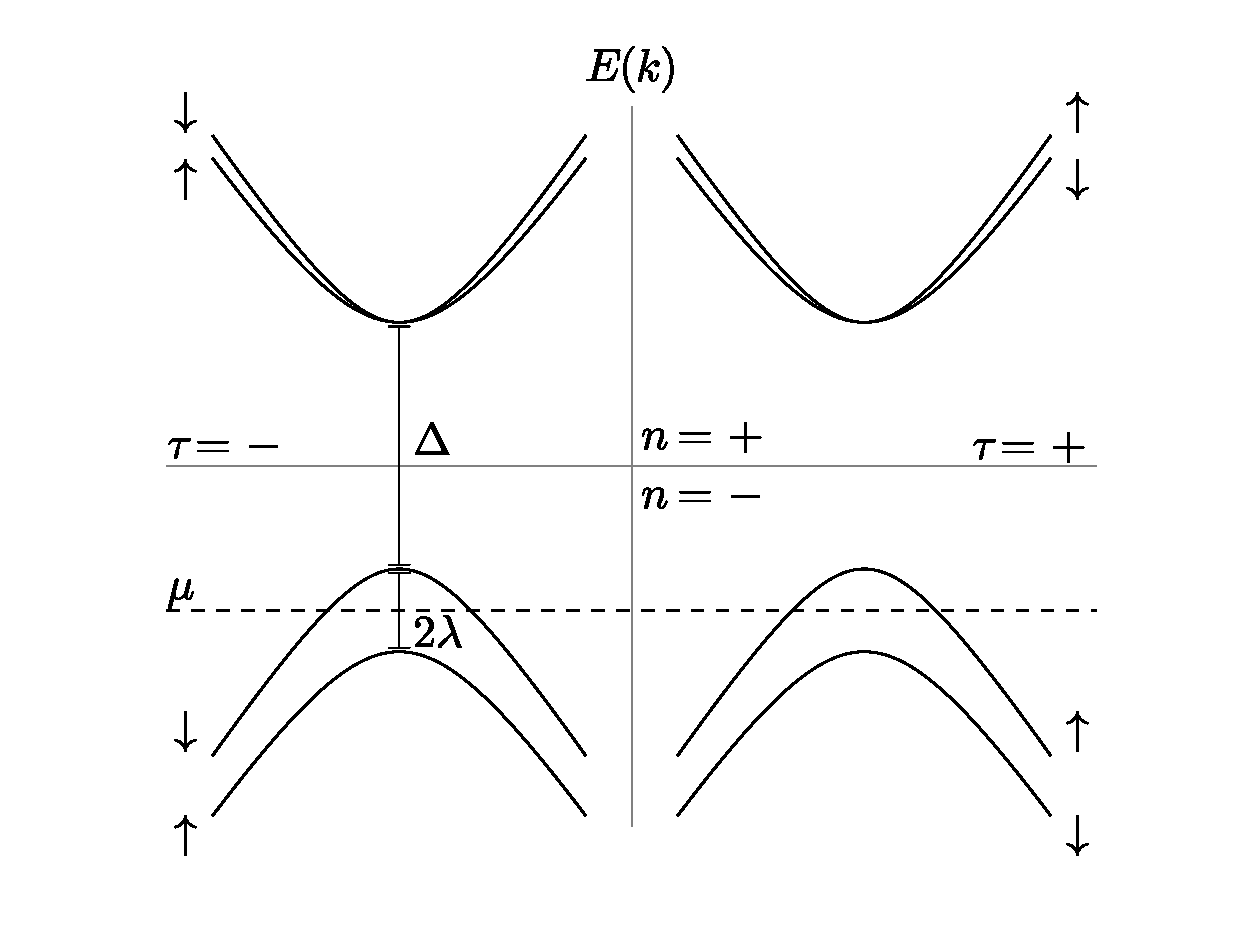
\includegraphics[width=\columnwidth]{figures/energy-bands}
  \caption{%
    Energy bands for $\ce{WSe2}$ as given by \cref{eq:energy}
    with $a t = \SI{3.939}{\electronvolt \per \angstrom}$,
    $Δ = \SI{1.60}{\electronvolt}$,
    and $λ = \SI{0.23}{\electronvolt}$.
    Each valley is centered at $± \vc{K}$ relative to the center of the
    Brillouin zone.
    The energy for a given band depends only on the distance $k$
    measured from the valley center.
  }\label{fig:energy}
\end{figure}

We focus on doped systems
such that the chemical potential $μ$ lies in the upper valence bands.
Within each band, the Bloch basis eigenstates are written
in terms of the orbital states as elements on the Block sphere,
\begin{equation}
  \Ket{u_{τ {\s}}^n \of{k, ϕ}}
  = \cos{\frac{\fnTheta{n}}{2}} \ketOrb{+}{\of{k, ϕ}}
  + e^{-i τ ϕ}
    \sin{\frac{\fnTheta{n}}{2}} \ketOrb{-}{\of{k, ϕ}},
\end{equation}
where $k_x + i τ k_y = k e^{i τ ϕ}$ and
\begin{equation}
  \tan{\frac{\fnTheta{n}}{2}}
  = \frac{a t τ k}{\dfrac{Δ}{2} - \fnEnergy{-n} \of{k}}
  = \frac{a t τ k}{\fnEnergy{n} \of{k} - \fnEnergy{-} \of{0}}.
\end{equation}
The polar angle on the Bloch sphere
of the conduction and valence bands are related by
$\fnTheta{-} - \fnTheta{+} = τ π$.
The mapping of the energy band to the Bloch sphere,
parametrized by $\left( θ, ϕ \right)$,
encodes the topological character:
as one moves from the node out to infinity,
the states sweep either the northern or southern hemisphere
with a chirality determined by the Berry curvature.

  \section{Superconductivity}

We consider two approaches to realizing a superconducting state.
First, we assume a proximity induced state obtained by
layering a TMD on an $s$-wave superconductor.
Second, we study an intrinsic correlated phase arising
from density-density interactions.

We use $d^ν_{τ {\s}} \ofK$ as the annihilation operator
for tight-binding $d$-orbital states,
and $c^n_{τ {\s}} \ofK$ for the eigenstates of the non-interacting Hamiltonian,
$λ_{\vK}$ for the energy dispersion for Bogoliubov quasiparticles,
and $Δ_{\vK}$ for the superconducting gap function.
A review of interaction theory may be found in \cref{s:appendix:interaction},
and additional computational detail for the intrinsic case
is given in \cref{s:appendix:tmdsc}.

\subsection{Induced State}

A proximity $s$-wave superconductor will inject Cooper pairs
according to
\begin{equation}
  H^V
  = ∑_{\vK, ν, τ} \cc{B}_ν
    d^ν_{-τ ↓} \ofMK d^ν_{τ ↑} \ofK + \frac{ε}{2} + \hc
\end{equation}
The coupling constants $B_ν$ and the overall constant $ε$
depend on the material interface%
\footnote{%
  Note that all sums over $\vK$ are restricted to $\left| \vK \right|$
  less than some cutoff that restricts the momentum to a single valley.
}.
Using the abbreviated notation
$c_{\vK α} = c^-_{τ {\s}} \ofK$,
with $α =\ ↑↓$ for $τ = {\s} = ±$,
projecting onto the upper valence bands yields,
\begin{align}
  \label{eq:induced}
  & P_{τ = {\s}}^{n = -} \left( H^0 + H^V - μ N \right) \\
  & = ∑_{\vK, α} ξ_{\vK} c_{\vK α}^† c_{\vK α}
    - \sumK \left( \cc{Δ}_{\vK} c_{-\vK ↓} c_{\vK ↑}
    + Δ_{\vK} c_{\vK ↑}^† c_{-\vK ↓}^† \right)
    + ε,
\end{align}
where $ξ_{\vK} = E_{+ ↑}^- \of{\abs{\vK}} - μ$ and
the effective BCS gap function is
\begin{equation}
  Δ_{\vK}
  = \frac{1}{2} \left( B_+ + B_- \right)
  + \frac{1}{2} \left( B_+ - B_- \right)
    \cos{θ_{\vK}},
\end{equation}
with $θ_{\vK} = θ_{+↑}^- \of{\abs{\vK}}$.%
\footnote{%
  We may take $Δ_{\vK}$ to be real.
  Otherwise, if $Δ_{\vK} = \abs{Δ_{\vK}} e^{i \arg{Δ_{\vK}}}$,
  then make the unitary transformation
  $c_{\vK α} → e^{i \arg{Δ_{\vK}} / 2} c_{\vK α}$.
}
This form is identical to the standard BCS Hamiltonian with
an effective spin index $α$.
However, the spin state of the Cooper pair is an equal superposition
of the singlet and the $m = 0$ component of spin triplet.
The corresponding quasiparticle eigenstates%
\footnote{%
  In this chapter we use $γ$ for these operators,
  however in the appendices, we use $b$ to avoid
  other notational conflicts.
}
are
$γ_{\vK α}
= α \cos{β_{\vK}} c_{\vK α} + \sin{β_{\vK}} c_{-\vK, -α}^†$,
with energies
$λ_{\vK} = ± \sqrt{ξ_{\vK}^2 + Δ_{\vK}^2}$,
where $\cos{2 β_{\vK}} = ξ_{\vK} / λ_{\vK}$.
Note that if $B_+ = B_-$,
then $Δ_{\vK}$ is a constant and independent of $\vK$.
Even when $B_+$ and $B_-$ are different,
the constant term dominates.
Before exploring the nature of this state,
we analyze the case of intrinsic superconductivity,
and show that the same state is energetically preferred.

\subsection{Intrinsic Phase}
\label{s:dichalcogenides:intrinsic}

For a local attractive density-density interaction
(e.g.\ one mediated by phonons), the potential is
$V ⋍ \frac{1}{2} ∑_{\vR, \vR'} v_{\vR \vR'}
\normalorder{n_{\vR} n_{\vR'}}$,
with $v_{\vR \vR'} = v_0 δ_{\vR \vR'}$
and $n_{\vR}$ the total Wannier electron density at lattice vector $\vR$.
Projecting onto states near the chemical potential gives
\begin{multline}
  \label{eq:channels}
  P_{τ = {\s}}^{n = -} \left( H^V \right)
  = \sumKK v \of{\vK' - \vK} \\
  × \left(
    A_{\vK \vK'}^2 c_{\vK' ↑}^† c_{-\vK' ↑}^† c_{-\vK ↑} c_{\vK ↑}
  + A_{\vK' \vK}^2 c_{\vK' ↓}^† c_{-\vK' ↓}^† c_{-\vK ↓} c_{\vK ↓}
    \right. \\ + \left.
      2 \abs{A_{\vK \vK'}}^2
      c_{\vK' ↑}^† c_{-\vK' ↓}^† c_{-\vK ↓} c_{\vK ↑}
    \vphantom{2 \abs{V_{\vK \vK'}}^2} \right),
\end{multline}
where
\begin{equation}
  A_{\vK \vK'}
  = e^{i \left( ϕ_{\vK'} - ϕ_{\vK} \right)}
    \sin{\frac{θ_{\vK'}}{2}} \sin{\frac{θ_{\vK}}{2}}
  + \cos{\frac{θ_{\vK'}}{2}} \cos{\frac{θ_{\vK}}{2}}.
\end{equation}
The first two terms in \cref{eq:channels} lead to intravalley pairing,
and the third to intervalley pairing.
We analyze the possible states within mean field theory.
The BCS order parameter is
\begin{equation}
  χ
  = v_0 \sumK \cc{g}_{\vK} \ev{c_{-\vK α'} c_{\vK α}},
\end{equation}
where the form of $g_{\vK}$ depends on the particular pairing channel.
The resulting Hamiltonian has the same form as the BCS Hamiltonian in
\cref{eq:induced}
but with an effective $Δ_{\vK} = g_{\vK} · χ$.
The intravalley pairing has three symmetry channels,
with the couplings given by
$2 g_{\vK} = 1 +  \cos{θ_{\vK}}$,
$\sqrt{2} e^{- i ϕ_{\vK}} g_{\vK} = \sin{θ_{\vK}}$
and $2 e^{- 2 i ϕ_{\vK}} g_{\vK} = 1 - \cos{θ_{\vK}}$.
For these channels, since
$\ev{c_{-\vK α} c_{\vK α}} = - \ev{c_{\vK α} c_{-\vK α}}$,
relabeling $\vK → -\vK$ in the sum gives $χ = 0$%
\footnote{%
  For odd parity interactions, where $v \ofMK = -v \ofK$, the
  intravalley pairing is not excluded by symmetry.
  Specifically, repeating the calculation with this assumption,
  the intervalley terms fully cancel, and one obtains \cref{eq:channels}
  without the intervalley term on the third line.
}.
The intervalley pairing also has three symmetry channels:
$g_{\vK} = \sqrt{2}$,
$g_{\vK} = \sqrt{2} \cos{θ_{\vK}}$,
and $g_{\vK} = \sqrt{2} \sin{θ_{\vK}} \vc{\hat{k}}$.
Of the three,
the constant valued channel is dominant%
\footnote{%
  For example, using the values for \ce{WSe2},
  $\sin^2 {θ_{\vK}} = 0.44$ and $\cos^2 {θ_{\vK}} = 0.56$
  at the chemical potential.
}.
This is to be expected, as the local density-density interaction
leads to the largest pairing for electrons of opposite spins.
Since the intravalley processes have the same spin,
they are disfavored as compared to the intervalley pairing.

The key features of the intrinsic superconducting state
are identical to the proximally induced case when density-density
interactions dominate.
We restrict further analysis to that case,
and turn to the question of optically induced pair-breaking phenomena.

  \section{Optoelectronic coupling}

The non-interacting system displays valley selective optical excitations.
Light of a particular polarization only couples to one valley.
Since the superconducting state is
a coherent condensate admixing the two valleys,
we address whether pair-breaking displays similar valley selectivity.
In particular, we explore whether or not the two quasiparticles generated
by circularly polarized light, with total energy larger than
$Δ + Δ_{\vK}$, occupy opposite valleys,
with one in the conduction band and the other in the valence band.

The optical excitations arise from the Berry curvature,
which acts as an effective angular momentum.
The electromagnetic potential $\vc{A}$,
with polarization vector $\vc{ϵ}$,
is introduced using minimal coupling,
$H_{τ {\s}}^{ν ν'} \ofK
→ H_{τ {\s}}^{ν ν'} \of{\vK + e \vc{A}}$,
where, in the dipole approximation,
$\vc{A} = 2 \re{\vc{ϵ} A_0 e^{- i ω t}}$.
This yields a perturbed Hamiltonian
$H → H + H^A$, where
$H^A = H' e^{- i ω t} + H'^† e^{i ω t}$,
with
\begin{equation}
  H'
  = ∑_{\vK, τ, {\s}}
    H'_τ
    {d^-_{τ {\s}}}^† \ofK
    d^+_{τ {\s}} \ofK
  - ∑_{\vK, τ, {\s}}
    H'_{-τ}
    {d^+_{τ {\s}}}^† \ofK
    d^-_{τ {\s}} \ofK,
\end{equation}
and
$H'_τ
= a t e A_0
\left( τ \vc{\hat{x}} + i \vc{\hat{y}} \right) · \vc{ϵ}$.
The transition rate is proportional to the modulus-squared
of the optical matrix elements,
$\vc{P}_{τ {\s}}^{n n'} \ofK$,
defined by
\begin{equation}
  H^A
  = ∑_{\substack{\vK, τ, {\s} \\ n, n'}}
    \frac{e A_0}{m_0}
    \vc{ϵ} · \vc{P}_{τ {\s}}^{n n'} \ofK
    {c_{τ {\s}}^n}^† \ofK
    c_{τ {\s}}^{n'} \ofK.
\end{equation}
For circularly polarized light, in the absence of superconductivity,
$\vc{ϵ}_± = \left( \vc{\hat{x}} ± i \vc{\hat{y}} \right) / \sqrt{2}$ and
\begin{equation}
  \label{eq:optical}
  \vc{ϵ}_± · \vc{P}_{τ {\s}}^{+ -} \of{\vK}
  = ∓ τ \sqrt{2} a t m_0
    e^{± i ϕ}
    \sin^2 {\frac{\fnTheta{∓ τ}}{2}}.
\end{equation}
See \cref{s:appendix:optical} for a full derivation.

\begin{figure}
  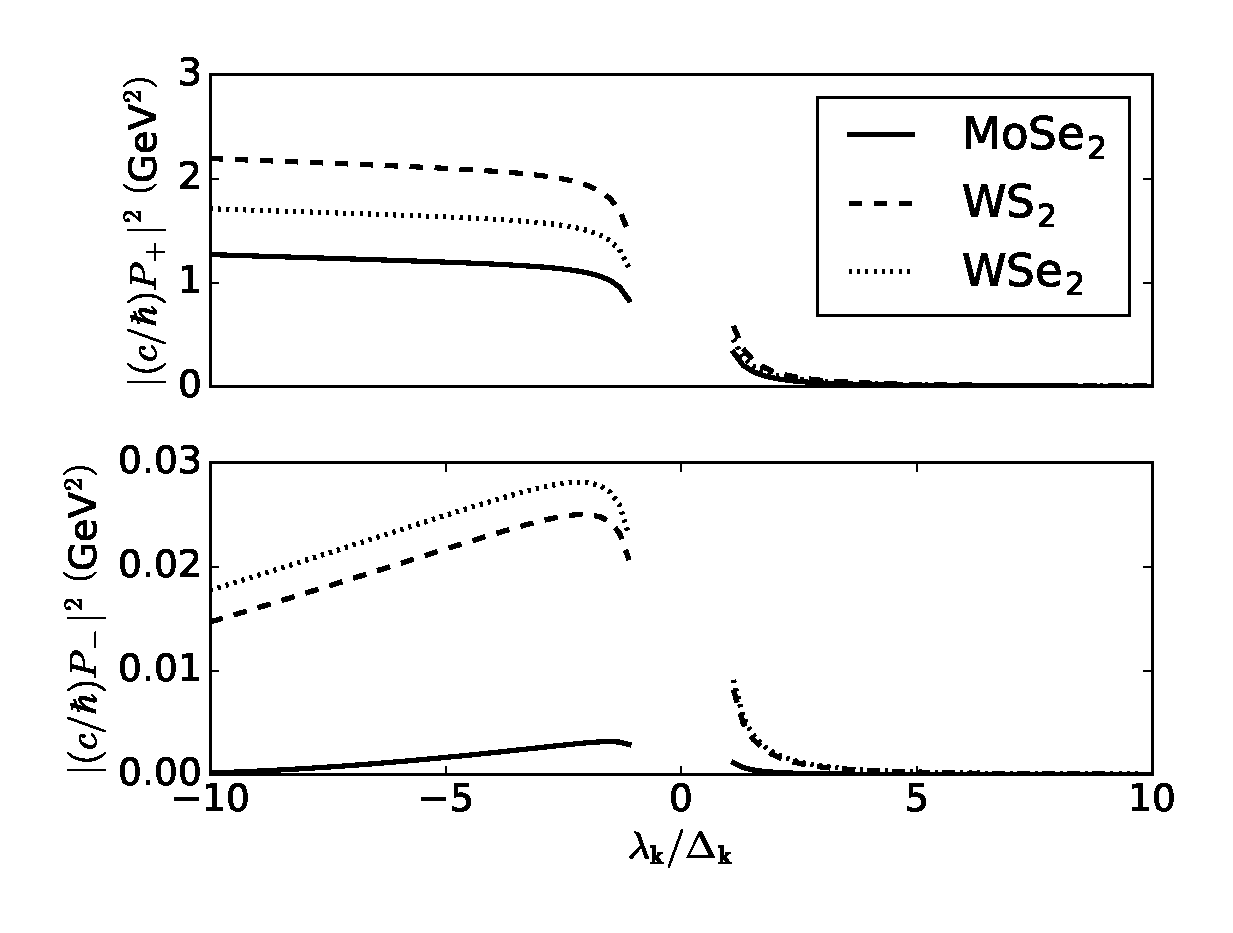
\includegraphics[width=\columnwidth]{figures/optical-transitions-bcs}
  \caption{%
    Optical transition rate matrix elements
    $\left| P_± \right|^2$
    in the superconducting phase
    as a function of the ratio of the quasiparticle energy
    $λ_{\vK}$ to the superconducting gap $Δ_{\vK}$.
    Material parameters for \ce{MoSe2}, \ce{WS2}, and \ce{WSe2}
    are given in~\cite{PhysRevLett.108.196802}
    and a gap of $Δ_{\vK} = \SI{7.5}{\milli\electronvolt}$
    is chosen for illustrative purposes.
    The order-of-magnitude contrast between
    $\left|P_+\right|^2$ and $\left|P_-\right|^2$
    causes the optical-valley selectivity.
  }\label{fig:optical}
\end{figure}

The transition rate matrix elements
for optical excitations from the BCS ground state
are given by \cref{eq:optical}
multiplied by a coherence factor $\sin {β_{\vK}}$.
Since $\fnTheta{-} - \fnTheta{+} = τ π$,
switching either the valley or polarization transforms
$\sin → \cos$ in \cref{eq:optical}, giving matrix elements
$\abs{P_±} = \abs{\vc{ϵ}_± · \vc{P}_{++}^{+ -} \ofK \sin {β_{\vK}}}$
corresponding to matching ($P_+$) or mismatching ($P_-$)
polarization-valley indexes.
For a given valley, a chosen polarization of light couples more strongly
than the other, as is evident comparing $\abs{P_+}^2$ to $\abs{P_-}^2$
and shown in \cref{fig:optical}.
For incident light with energy $Δ + \abs{λ_{\vK}}$,
right circularly polarized light ($+$) has a higher probability
of promoting a quasiparticle to the right conduction band,
as reflected in the larger matrix element $\abs{P_+}^2 ≫ \abs{P_-}^2$.
As depicted in \cref{fig:optical-excitation},
the partner of the Cooper pair is in the valence band in the opposite valley.
The other valley has the opposite dependence on polarization.

This key new result opens the door for valley control of excitations
from a coherent ground state.
For example, the two quasiparticles have the same charge and Berry curvature
(see below).
In the presence of an electric filed,
they both acquire the same transverse anomalous velocity.
Thus, in contrast to the response in the normal state,
an anomalous Hall effect is anticipated
with no accompanying spin current.

\begin{figure}
  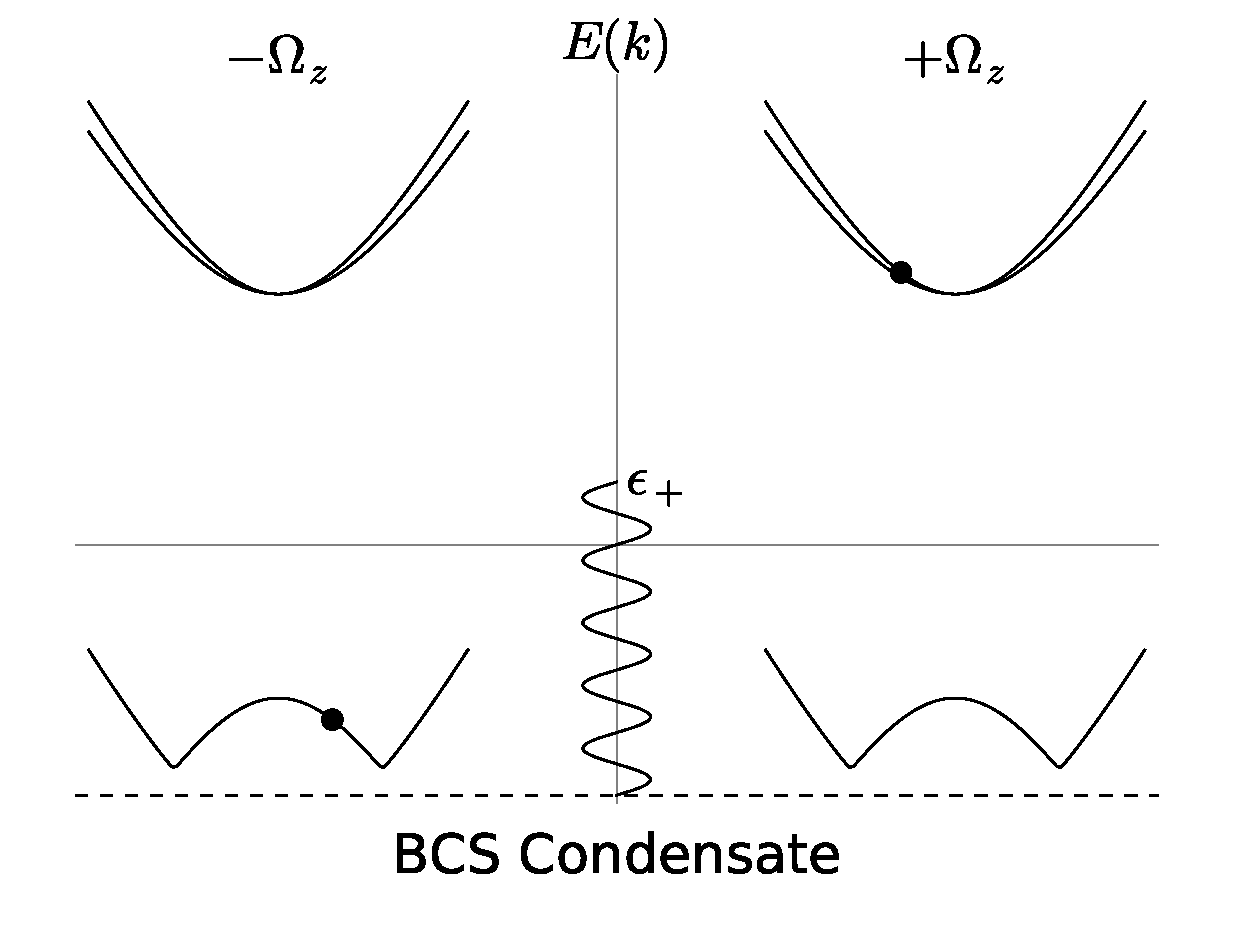
\includegraphics[width=\columnwidth]{figures/bcs-excitation}
  \caption{%
    Pair-breaking by right circularly polarized light
    leads to an electron in the conduction band of the right valley
    and a partner in the valence band of the left valley.
    The valleys interchange for left circularly polarized light.
  }\label{fig:optical-excitation}
\end{figure}

  \section{Berry curvature}

The Berry curvature in the non-interacting crystal
for left and right circularly polarized
($\vc{ϵ}_±$) optical excitations for a given $\vK$
is $± 2 Ω_{+ ↑}^+ \of{k}$, where
\begin{subequations}
  \begin{align}
    Ω_{τ {\s}}^n \of{k}
    & = \vc{\hat{z}} · \vc{Ω}_{τ {\s}}^n \ofK, \\
    & = - n τ
        \left[ \frac{1}{2 k} \pderiv{}{k} \fnTheta{n} \right]
        \sin{\fnTheta{n}}, \\
    & = - n τ
        \frac{2 {\left( a t \right)}^2 \left( Δ - λ τ {\s} \right)}
        {{\left[{\left( 2 a t k \right)}^2
      + {\left( Δ - λ τ {\s} \right)}^2 \right]}^{3/2}}.
  \end{align}
\end{subequations}

The BCS ground state is%
\footnote{%
  Note that the full ground state
  also contains the two lower filled bands,
  but those contribute zero net Berry curvature and may be ignored
  in this section and the next.
}
\begin{subequations}
  \begin{align}
    \Ket{Ω}
    & = ∏_{\vK} \csc{β_{\vK}} γ_{\vK ↑} γ_{-\vK ↓} \Ket{0}, \\
    & = ∏_{\vK} \left( \cos{β_{\vK}} - \sin{β_{\vK}}
        c_{\vK ↑}^† c_{-\vK ↓}^† \right) \Ket{0}.
  \end{align}
\end{subequations}
This superconducting state is built up
from the quasiparticle eigenstates,
$\Ket{\vK}
= \csc{β_{\vK}} γ_{\vK ↑} γ_{-\vK ↓} \Ket{0}$,
of the $\vK$-dependent Hamiltonian
$λ_{\vK} \left( γ_{\vK ↑}^† γ_{\vK ↑}
+ γ_{-\vK ↓}^† γ_{-\vK ↓} \right)$.
The $z$-component of the Berry curvature of
the correlated state is zero,
\begin{equation}
  \vc{\hat{z}} · i ∇_{\vK} ⨯
  \Braket{\vK | ∇_{\vK} | \vK}
  = Ω_{+ ↑}^- \of{k} + Ω_{- ↓}^- \of{-k} = 0.
\end{equation}
A single optically excited state in the left valley
for a given $\vK$ is
${c_{+ ↑}^+}^† \ofK c_{+ ↑}^- \Ket{\vK}$,
which has a Berry curvature
$+2 \sin^6 {β_{\vK}} Ω_{+ ↑}^+ \of{k}$.
The corresponding excitation in the right valley
has a Berry curvature of the same magnitude but opposite sign.

  \section{Conclusions}

In this letter, we report on the nature of the superconducting state
of hole-doped TMDs.
Remarkably, the correlated state inherits
the valley contrasting phenomena of the parent state.
While the magnitude is smaller, pair-breaking produces quasiparticles
that have the same Berry curvature, and hence the same anomalous velocity.
Thus, one predicts an anomalous Hall response similar to
the one observed in \ce{MoSe2}.
Further consequences of the phenomena will be explored elsewhere.

Spin-valley locking leads to large critical magnetic fields.
A similar phenomena was recently reported in heavily hole-doped
(beyond the spin-split gap) \ce{NbSe2}
\cite{%
  1510.06289v2,%
  PhysRevLett.113.097001%
}.
In the new regime, where only one band per valley intersects
the chemical potential, no pair-breaking occurs
for in-plane fields unless disorder is present.

While systematic synthesis and characterization of hole-doped systems
is still in its early stages, the fact that other two-dimensional compounds
and their bulk counterparts are known to be superconducting
\cite{%
  PhysRevB.88.054515%
}
provides impetus to explore the novel phenomena described here.

  \section{Acknowledgments}

The software developed %
\footnote{%
  Related software and source code at \\
  \url{https://evansosenko.com/dichalcogenides/}
}
and used~\cite{Hunter:2007} for this work
and the included figures is available freely online.
We thank Michael Phillips for useful discussions.
We acknowledge the support of the Army Research Office through the grant
ARO W911NF1510079.


  \chapter{TMD SC Background}
  \section{Essential Physics}
\label{s:appendix}

In this appendix, we review the essential physical theory
underlying our model and computations.

\subsection{Optical Transitions}

Consider the spin-orbit Hamiltonian for a single non-interacting electron
which includes a position dependent potential $W \of{\vc{Q}}$
and an electromagnetic potential $\vc{A} \of{\vc{Q}}$,
\begin{equation}
  H = \frac{{\left( \vc{P} + e \vc{A} \right)}^2}{2 M}
      + λ \vc{L} · \vc{S} + W.
\end{equation}
Given $\vc{L} = \vc{Q} × \vc{P}$, one can show, either via
the commutation relations or formal differentiation,
that the velocity operator is
\begin{equation}
  \vc{V}
  = i [H, \vc{Q}] = \pderiv{H}{\vc{P}}
  = \frac{\vc{P} + e \vc{A}}{M} + λ \vc{Q} × \vc{S}.
\end{equation}

In a gauge with $∇ ·\vc{A} = 0$,
\begin{equation}
  H = \frac{\vc{P}^2}{2 M} + \frac{e}{M} \vc{A} · \vc{P} + e^2 \vc{A}^2.
\end{equation}

For monochromatic optical perturbations
with wave vector $\vc{q}$, frequency $ω$, and polarization vector $\vc{ϵ}$,
the electromagnetic potential is of the form
$\vc{A} = 2 \re{\vc{ϵ} A_0 e^{i \left( \vc{q} · \vc{Q} - ω t \right)}}$.
For linear perturbations, we neglect the term of order $\vc{A}^2$
to write the Hamiltonian in the form
$H = H_0 + H' e^{- i ω t} + {H'}^† e^{i ω t}$.
Here,
$H' = e A_0 e^{i \vc{q} · \vc{Q}} \left( \vc{ϵ} · \vc{V} \right)$
appears as a standard harmonic perturbation where
$\vc{V} = i [ H_0, \vc{Q} ]$
is the velocity operator for the unperturbed system.

Thus, according to Fermi's golden rule,
the optical transition probability per unit time is
\begin{equation}
  Γ_{f ← i}
  = 2 π e^2 A_0^2
    \abs{\Braket{f | e^{i \vc{q} · \vc{Q}} \vc{ϵ} · \vc{V} | i}}^2
    δ \of{E_f + E_i - ω}. % chktex 19
\end{equation}
Typically, the dipole approximation is used in which
$e^{i \vc{q} · \vc{Q}} → 1$.

\subsection{Transition Operators}

We first define the position-space translation operator,
$T \of{\vc{r}} = e^{- i \vc{r} · \vc{P}}$,
and the momentum-space translation operator
$T_{\vK} = e^{- i \vc{k} · \vc{Q}}$.
We assume zero magnetic field.%
\footnote{%
  For nonzero field, however, much of the following can be recast
  in terms of the magnetic translation operators.
  % TODO Add references.
}
Each has a simple inverse:
$T^{-1} \of{\vc{r}} = T \of{- \vc{r}}$
and
$T_{\vK}^{-1} = T_{- \vK}$.
We also note the derivatives:
$∇_{\vK} T_{\vK} = - i \vc{Q} T_{\vK}$
and
$∇_{\vK} T^{-1}_{\vK} = i \vc{Q} T^{-1}_{\vK}$.

We can compute a useful commutation relation of these translations operators.
Application of the Baker–Campbell–Hausdorff formula gives
\begin{subequations}
  \begin{align}
    T \of{\vc{r}} T_{\vK}
      & = e^{- i \left( \vc{r} · \vc{P} + \vc{k} · \vc{Q} \right)
          - \frac{1}{2} \left[ \vc{r} · \vc{P}, \vc{k} · \vc{Q} \right]}, \\
    %
    T_{\vK} T \of{\vc{r}}
      & = e^{- i \left( \vc{r} · \vc{P} + \vc{k} · \vc{Q} \right)
          + \frac{1}{2} \left[ \vc{r} · \vc{P}, \vc{k} · \vc{Q} \right]}.
  \end{align}
\end{subequations}
Only a single commutator appears above since
$\left[ \vc{r} · \vc{P}, \vc{k} · \vc{Q} \right] = - i \vc{r} · \vc{k}$,
and substituting this in above we see
\begin{equation}
  \label{eq:translations:commutation}
  T \of{\vc{r}} T_{\vK}
  = e^{-i \vc{r} · \vc{k}} T_{\vK} T \of{\vc{r}}.
\end{equation}

\subsection{Bloch Hamiltonian}

Given a Hamiltonian $H$ and a set of $N$ lattice vectors
$\left\{ \vRn{n} \right\}$ such that the Hamiltonian
commutes with each $T \of{\vRn{n}}$,
we may choose a set of common eigenvectors according to Bloch's theorem,
\begin{subequations}
  \begin{align}
    H \Ket{ψ_{n \vK}}
      & = E_{n \vK} \Ket{ψ_{n \vK}}, \\
    T \of{\vRn{m}} \Ket{ψ_{n \vK}}
      & = e^{-i \vK · \vRn{m}} \Ket{ψ_{n \vK}}.
  \end{align}
\end{subequations}
Given periodic boundary conditions,
the set of allowed $\vK$ becomes countable
and may be restricted to the first Billouin zone
due to the periodicity of the eigenvalues
with respect to translation by a reciprocal lattice vector $\vG$.
For each $\vK$, the transformation
$\Ket{u_{n \vK}} = T_{\vK} \Ket{ψ_{n \vK}}$
gives a set of states which are invariant under lattice translations, i.e.,
using \cref{eq:translations:commutation},
$T \of{\vRn{m}} \Ket{u_{n \vK}} = \Ket{u_{n \vK}}$.
A general operator then transforms according to
$A_{\vK}~=~T_{\vK} A T_{\vK}^{-1}$.
In particular,
\begin{align}
  H_{\vK}
    & = ∑_{n \vK'} E_{n \vK'} T_{\vK} \Ket{ψ_{n \vK'}}
        \Bra{ψ_{n \vK'}} T_{\vK}^{-1}, \\
    & = H_{\vK}^0 + H_{\vK}^1,
\end{align}
where
\begin{subequations}
  \begin{align}
    \label{eq:a:h.bloch.terms}
    H_{\vK}^0
      & = ∑_n E_{n \vK} \Ket{u_{n \vK}} \Bra{u_{n \vK}}, \\
    H_{\vK}^1
      & = ∑_n ∑_{\vK' ≠ \vK} E_{n \vK'} T_{\vK - \vK'}
          \Ket{u_{n \vK'}} \Bra{u_{n \vK'}} T_{\vK - \vK'}^{-1}.
  \end{align}
\end{subequations}

Note that the derivative of a transformed operator may be computed as
\begin{equation}
  ∇_{\vK} A_{\vK}
    = ∇_{\vK} \left( T_{\vK} A T_{\vK}^{-1} \right)
    = i \left[ A_{\vK}, \vc{Q} \right].
\end{equation}
In particular,
\begin{equation}
  ∇_{\vK} H_{\vK} = \vc{V}_{\vK}.
\end{equation}
Thus, for each $\vK$,
the matrix element appearing in the optical transition rate
(in the dipole approximation) may be computed as
\begin{equation}
  \Braket{ψ_{n' \vK} | \vc{V} | ψ_{n \vK}}
  = \Braket{u_{n' \vK} | \vc{V}_{\vK} | u_{n \vK}}
  = \Braket{u_{n' \vK} | ∇_{\vK} H_{\vK} | u_{n \vK}}.
\end{equation}

\subsection{Tight Binding Model}

In the tight biding model, one assumes there exists a finite set
$\left\{ \Ket{φ_ν} \right\}$ of relevant atomic orbitals.
The corresponding Bloch orbital states,
\begin{equation}
  \Ket{ϕ_{ν \vK}}
  = \frac{1}{\sqrt{N}}
    ∑_{n = 1}^N e^{i \vK ⋅ \vRn{n}}
    T \of{\vRn{n}} \Ket{φ_ν},
\end{equation}
provide a complete bases for the space
of Bloch eigenstates $\left\{ \Ket{ψ_{n \vK}} \right\}$, i.e.,
\begin{subequations}
  \begin{align}
    \Ket{ψ_{n \vK}} & = ∑_ν M_{\vK}^{ν n} \Ket{ϕ_{ν \vK}}, \\
    \Ket{ϕ_{ν \vK}} & = ∑_n W_{\vK}^{n ν} \Ket{ψ_{n \vK}},
  \end{align}
\end{subequations}
with $M_{\vK}^{ν n} = \cc{W}_{\vK}^{ν n}$.
The second overlap term in
\begin{equation}
  \Braket{ϕ_{ν' \vK} | ϕ_{ν \vK}}
  = \Braket{φ_{ν'} | φ_ν}
    + ∑_{\vRn{n} ≠ 0}^N e^{i \vK ⋅ \vRn{n}}
    \Braket{φ_{ν'} | T \of{\vRn{n}} | φ_ν},
\end{equation}
is small, thus the states
$\left\{ \Ket{φ_ν} \right\}$ are assumed formally orthonormal.

Since each $\Ket{ϕ_{n k}}$ satisfies
\begin{equation}
  T \of{\vRn{m}} \Ket{ϕ_{ν \vK}}
  = e^{-i \vK · \vRn{m}} \Ket{ϕ_{ν \vK}},
\end{equation}
the transformed orbital states
$\Ket{v_{n \vK}} = T_{\vK} \Ket{ϕ_{n k}}$
are invariant under lattice translations.
One typically knows the matrix elements
of an effective Hamiltonian
in the bases of these periodic Bloch orbitals,
\begin{equation}
  H_{\vK}^{ν ν'}
  = \Braket{v_{ν \vK} | H_{\vK} | v_{ν' \vK}}
  = ∑_n \cc{W}_{\vK}^{n ν} E_{n \vK} W_{\vK}^{n ν'},
\end{equation}
which determines the coefficients $M_{\vK}^{ν n}$.

\subsubsection{Optical Matrix Elements}

The matrix elements of the derivative,
$\Braket{u_{n \vK} | ∇_{\vK} H_{\vK} | u_{n' \vK}}$,
appearing in the optical translation rate may be cumbersome to compute.
We show that in the tight binding approximation with only $d$-type orbitals,
it is sufficient to compute the derivative of the orbital matrix elements,
$∇_{\vK} H_{\vK}^{ν ν'}
= ∇_{\vK} \Braket{v_{ν \vK} | H_{\vK} | v_{ν' \vK}}$.

We may write \cref{eq:a:h.bloch.terms} as
\begin{align}
  \label{appendix:optical:decomposition}
  H_{\vK}^0
  & = ∑_{ν, ν'}
      H_{\vK}^{ν ν'}
      \Ket{v_{ν \vK}} \Bra{v_{ν' \vK}}, \\
  H_{\vK}^1
  & = ∑_{ν, ν'} ∑_{\vK' ≠ \vK}
      H_{\vK'}^{ν ν'}
      T_{\vK - \vK'}
      \Ket{v_{ν \vK'}} \Bra{v_{ν' \vK'}}
      T_{\vK - \vK'}^{-1}.
\end{align}
First, using
$∇_{\vK} H_{\vK}^1 = i \left[ H_{\vK}^1, \vc{Q} \right]$,
we obtain a sum over $\vK' ≠ \vK$ of terms proportional
to $δ_{\vK, \vK'}$, % chktex 19
thus all matrix elements for $∇_{\vK} H_{\vK}^1$ vanish.
Next, we have
\begin{multline}
  \label{appendix:optical:sum}
  ∇_{\vK} H_{\vK}^0
  = ∑_{ν, ν'}
    ∇_{\vK} H_{\vK}^{ν ν'}
    \Ket{v_{ν \vK}} \Bra{v_{ν' \vK}} \\
  + ∑_{ν, ν'}
    H_{\vK}^{ν ν'}
    \left( ∇_{\vK} \Ket{v_{ν \vK}} \right) \Bra{v_{ν' \vK}} \\
  + ∑_{ν, ν'}
    H_{\vK}^{ν ν'}
    \Ket{v_{ν \vK}} \left( ∇_{\vK}  \Bra{v_{ν' \vK}} \right).
\end{multline}
Using
\begin{equation}
  \label{appendix:optical:ket:del}
  ∇_{\vK} \Ket{v_{ν \vK}}
  = \frac{T_{\vK}}{i \sqrt{N}}
    ∑_{n = 1}^N e^{i \vK ⋅ \vRn{n}}
    T \of{\vRn{n}} \vc{Q} \Ket{φ_ν},
\end{equation}
we find the second sum in
\cref{appendix:optical:sum}
contains terms proportional to the local optical matrix elements,
$\Braket{φ_ν' | T \of{\vRn{n}} \vc{Q} | φ_ν}$.
For finite $\vRn{n}$, these off-center integrals are small,
and for $\vRn{n} = 0$, optical transitions between $d$-orbitals
are forbidden by symmetry.
Similar logic applies to the third sum in
\cref{appendix:optical:sum},
thus
\begin{equation}
  \label{appendix:optical:approx}
  \Braket{u_{n \vK} | ∇_{\vK} H_{\vK} | u_{n' \vK}}
  ⋍ ∑_{ν, ν'}
    \cc{M}_{τ σ}^{ν n} \ofK
    \left( ∇_{\vK} H_{\vK}^{ν ν'} \right)
    M_{τ σ}^{ν' n'} \ofK
\end{equation}

  \subsection{Electron-Electron Interaction}

The BCS theory of superconductivity is often introduced as
a consequence of the effective electron-electron interaction
arising from the underlying electron-phonon interaction.
In this section, we review general two particle interactions,
and derive the form of the electron-electron interaction
when applied to the tight binding model.

Consider a general spin-independent interaction potential
$v \of{\vc{x}, \vc{x}'}$ which depends on the positions
$\vc{x}$ and $\vc{x}'$ of a pair of particles.
In a multiparticle system of dimension $d$ with no self-interaction,
this may be written as an additive pair operator
in a given bases of fermionic Fock operators,
$C_α^† \Ket{0} = \Ket{α} = \Ket{f_α} ⊗ \Ket{σ_α}$, as
% TODO Cite Ballentine, etc..

\begin{equation}
  \label{eq:interaction:general}
  \begin{aligned}
  V
  & = \frac{1}{2} ∑_{i ≠ j} v \of{\vc{Q}_i, \vc{Q}_j}, \\
  & = \frac{1}{4} \sumInt
    \Braket{α β | v | γ δ} C_α^† C_β^† C_δ C_γ, \\ % chktex 19
  & = \frac{1}{2} \sumInt
    v_{α β, γ δ} C_α^† C_β^† C_δ C_γ. % chktex 19
  \end{aligned}
\end{equation}
Here, $\Ket{α β} = \left( \Ket{α} \Ket{β}
- \Ket{β} \Ket{α} \right) / \sqrt{2}$,
and we introduce the symbol
\begin{multline}
  v_{α β, γ δ} % chktex 19
  = \left( \Bra{f_α} \Bra{f_β} \right) v
    \left( \Ket{f_γ} \Ket{f_δ} \right) % chktex 19
    \Braket{σ_α | σ_γ} \Braket{σ_β | σ_δ}, \\ % chktex 19
  = δ_{σ_α σ_γ} δ_{σ_β σ_δ} % chktex 19
    ∫ \cc{f}_α \of{\vc{x}} \cc{f}_β \of{\vc{x}'} v % chktex 19
    \of{\vc{x}, \vc{x}'} f_γ \of{\vc{x}} f_δ \of{\vc{x}'} % chktex 19
    \dif^d \vc{x} \dif^d \vc{x}',
\end{multline}
so that $\Braket{α β | v | γ δ} = v_{α β, γ δ} - v_{α β, δ γ}$. % chktex 19

If one chooses the continuous basis of position eigenstates,
$Ψ_σ^† \of{\vc{x}} \Ket{0} = \Ket{\vc{x}} ⊗ \Ket{σ}$,
then \cref{eq:interaction:general} takes the form of an integral over
density-density interactions,
\begin{equation}
  \label{eq:interaction:position-space}
  V
  = \frac{1}{2}
    ∫ v \of{\vc{x}, \vc{x}'}
    \normalorder{ρ \of{\vc{x}} ρ \of{\vc{x}'}}
    \dif^d \vc{x} \dif^d \vc{x}',
\end{equation}
where the colon denotes normal ordering and
\begin{equation}
  ρ \of{\vc{x}} = ∑_σ Ψ_σ^† \of{\vc{x}} Ψ_σ \of{\vc{x}}.
\end{equation}

For interactions which depend only on the relative separation,
$v \of{\vc{x}, \vc{x}'} = v \of{\vc{x}' - \vc{x}} = v \of{\vc{r}}$,
if one chooses the countable basis
of box normalized momentum eigenstates in a volume $Ω$
with periodic boundary conditions,
$c_{\vc{p} σ}^† \Ket{0} = \Ket{\vc{p}} ⊗ \Ket{σ}$
with
$\Braket{\vc{x} | \vc{p}} = Ω^{-1 / 2} e^{i \vc{p} · \vc{x}}$
then
\begin{equation}
  \label{eq:interaction:momentum-space}
  V
  = \frac{1}{2}
    ∑_{\vc{p}, \vc{p'}, \vc{q}}
    ∑_{σ, σ'}
    \tilde{v}_{\vc{q}}
    c_{\vc{p} + \vc{q} σ}^† c_{\vc{p}' - \vc{q} σ'}^†
    c_{\vc{p}' σ'} c_{\vc{p} σ},
\end{equation}
where
\begin{equation}
  \label{eq:interaction:fourier:coefficients}
  \tilde{v}_{\vc{q}}
  = \frac{1}{Ω} ∫ v \of{\vc{r}} e^{-i \vc{q} · \vc{r}} \dif^d \vc{r}.
\end{equation}

\subsubsection{Interaction in the Tight Binding Model}

We now apply the above to the basis introduced in the tight binding model.
Introduce a Wannier representation,
\begin{equation}
  \Ket{ϕ_{ν \vK}}
  = \frac{1}{\sqrt{N}}
    ∑_{\vR} e^{i \vK ⋅ \vR}
    \Ket{ϕ_{ν \vR}},
\end{equation}
where for convenience we write $\vR$ for $\vRn{n}$.
We adopt the following section-specific notation for the Fock operators,
\begin{subequations}
  \begin{alignat}{2}
    a_{\vK ν σ}^† \Ket{0}
    &  = \Ket{ϕ_{ν \vK σ}}
    && = \Ket{ϕ_{ν \vK}} ⊗ \Ket{σ}, \\
    a_{\vR ν σ}^† \Ket{0}
    &  = \Ket{ϕ_{ν \vR σ}}
    && = \Ket{ϕ_{ν \vR}} ⊗ \Ket{σ}.
  \end{alignat}
\end{subequations}
which explicitly separates out the spin index.
Since
\begin{equation}
  \Braket{\vc{x} | ϕ_{ν \vR}}
  = \Braket{\vc{x} - \vR | φ_ν}
  = φ_ν \of{\vc{x} - \vR},
\end{equation}
by keeping only on-center, like-orbital terms,
the interaction may by simplified to the approximate form
\begin{equation}
  V
  ⋍ \frac{1}{2}
    ∑_{\vR, \vR'}
    ∑_{ν, ν'}
    v_{\vR \vR'}^{ν ν'}
    \normalorder{n_{\vR ν} n_{\vR' ν'}},
\end{equation}
with the number operators,
\begin{equation}
  n_{ν \vR}
  = ∑_σ a_{\vR ν σ}^† a_{\vR ν σ},
\end{equation}
and interaction integral,
\begin{equation}
  v_{\vR \vR'}^{ν ν'}
  = ∫ v \of{\vc{x}, \vc{x}'}
    \abs{φ_ν \of{\vc{x} - \vR}}^2
    \abs{φ_{ν'} \of{\vc{x}' - \vR'}}^2
    \dif^d \vc{x} \dif^d \vc{x}'.
\end{equation}
This sum over density-density interactions mimics
\cref{eq:interaction:position-space}.

Further, assuming that the interaction
depends only on the relative separation,
$v_{\vR \vR'}^{ν ν'} = v_{ν ν'} \of{\vR' - \vR}$,
we may introduce the Fourier expansion
\begin{equation}
  \tilde{v}^{ν ν'}_{\vc{q}}
  = ∑_{\vR} v_{ν ν'} \of{\vR} e^{i \vc{q} · \vR},
\end{equation}
and switch back to the Bloch representation,
\begin{multline}
  \label{eq:interaction:tight-binding:momentum}
  V
  = \frac{1}{2} {\left( \frac{Ω}{N} \right)}^2
    ∑_{ν, ν'}
    ∑_{σ, σ'}
    ∑_{\vK', \bar{\vK}}
    ∑_{\vK, \bar{\vK}'}
    ∑_{\vc{q}}
    \tilde{v}^{ν ν'}_{\vc{q}} \\
    δ \left[ \vc{q} - \left(\vK - \bar{\vK} \right) \right] % chktex 19
    δ \left[ \vc{q} - \left(\bar{\vK}' - \vK' \right) \right] \\ % chktex 19
    a_{\bar{\vK} ν σ}^† a_{\bar{\vK}' ν' σ'}^†
    a_{\vK' ν' σ'} a_{\vK ν σ}.
\end{multline}
As a convenience, we have written this
as a sum over a countable set of momentum states,
however any sum over momentum may be converted to an integral
according to the substitution
$∑_{\vK} → \left( N / Ω \right) ∫ \dif^d \vK$.
Using this, we may integrate out the $δ$-functions % chktex 19
and obtain a form that mimics
\cref{eq:interaction:momentum-space},
\begin{equation}
  \label{eq:interaction:tight-binding:final}
  V
  = \frac{1}{2}
    ∑_{\vK, \vK', \vc{q}}
    ∑_{ν, ν'}
    ∑_{σ, σ'}
    \tilde{v}^{ν ν'}_{\vc{q}}
    a_{\vK + \vc{q} ν σ}^† a_{\vc{\vK' - \vc{q}} ν' σ'}^†
    a_{\vK' ν' σ'} a_{\vK ν σ}.
\end{equation}

  \section{Dichalcogenide System}
\label{appendix:model}

\subsection{Model}

The minimal model
\cite{PhysRevLett.108.196802}
for single-layer TMDCs in the low energy bands
about the $± \vc{K}$ points is a two-band tight binding model with bases
\begin{subequations}
\label{eq:orbitals}
  \begin{alignat}{2}
    & \ketOrbital{\text{c}} && = \Ket{d_{z^2}} ⊗ \Ket{σ}, \\
    & \ketOrbital{\text{v}} && = \frac{1}{\sqrt{2}}
        \left( \Ket{d_{x^2 - y^2}} + i τ \Ket{d_{xy}} \right) ⊗ \Ket{σ}.
  \end{alignat}
\end{subequations}
Here, $\Ket{σ}$ is the spin state,
and $\Ket{d_{xy}}$ and $\Ket{d_{x^2 - y^2}}$
refer to the angular momentum orbitals
in the symmetry group $E \left( d_{xy}, d_{x^2 - y^2} \right)$.
The valley index $τ = ±1$, corresponding to the $± \vc{K}$ points,
and the spin index $σ = ±1$ (or $σ = ↑,↓$), corresponding to the $z$-component
of the spin through $s_z = σ / 2$, are good quantum numbers.
The periodic Bloch basis states
(see \cref{s:appendix}) are
\begin{equation}
  \ketOrbitalK{ν}
  = \frac{T_{\vK +  τ \vc{K}}}{\sqrt{N}}
    ∑_{n = 1}^N e^{i \left( \vK + τ \vc{K} \right) ⋅ \vRn{n}}
    T \of{\vRn{n}} \ketOrbital{ν},
\end{equation}
where $ν = \text{c}, \text{v}$ is the orbital basis index
and $N$ is the number of \ce{M}-type atoms in the system.

The effective Bloch Hamiltonian is
\begin{multline}
  \label{eq:hamiltonian:effective}
  H_τ^0 \ofK
  = a t \left(τ k_x σ_x + k_y σ_y \right) ⊗ I_2 \\
    + \frac{Δ}{2} σ_z ⊗ I_2 - λ τ \left(σ_z - 1 \right) ⊗ S_z,
\end{multline}
where $Δ$ is the energy gap, $2 λ$ is the spin splitting in the lower band,
$a$ is the lattice constant, and $t$ is the effective hopping integral.
Note that $Δ > 2 λ$.
The operators $σ_i$ are Pauli operators acting on the orbital space
such that $σ_z \ketOrbitalK{\text{c}} = \ketOrbitalK{\text{c}}$
and $σ_z \ketOrbitalK{\text{v}} = - \ketOrbitalK{\text{v}}$.
\Cref{eq:hamiltonian:effective}
can be written in matrix form in the Bloch orbital basis,
\begin{equation}
  \left[ H_{τ σ}^0 \ofK \right] =
    \left[
    \begin{matrix}
      \dfrac{Δ}{2}                     & a t \left( τ k_x - i k_y \right) \\
      a t \left( τ k_x + i k_y \right) & λ τ σ - \dfrac{Δ}{2}
    \end{matrix}
    \right].
\end{equation}

\subsubsection{Energy}

The Hamiltonian is diagonal in all but the binary orbital index,
thus the eigenstates may be written as elements of a Bloch sphere,
\begin{equation}
  \begin{aligned}
    \ketEigenstateKPhi{n} =
                   & \cos{\frac{\fnTheta{n}}{2}} \ketOrbitalKPhi{c} \\
      + e^{-i τ ϕ} & \sin{\frac{\fnTheta{n}}{2}} \ketOrbitalKPhi{v},
  \end{aligned}
\end{equation}
where $k_x + i τ k_y = k e^{i τ ϕ}$,
$k = \abs{\vK}$, and
\begin{equation}
  \tan{\frac{\fnTheta{n}}{2}}
  = \frac{a t τ k}{\dfrac{Δ}{2} - \fnEnergy{-n} \of{k}}
  = \frac{a t τ k}{\fnEnergy{n} \of{k} - \fnEnergy{-} \of{0}}.
\end{equation}
Note the relations
$θ_{-↓}^{n} \of{k} = 2π - θ_{+↑}^{n} \of{k}$,
$\fnTheta{+} = \fnTheta{-} - τ π$,
and $ϕ_{-\vK} = π + ϕ_{\vK}$.
We will primarily write equations in terms of
$θ_{\vK} = θ_{+↑}^- \of{\abs{\vK}}$.
The energies are given by
\begin{equation}
  \fnEnergy{n} \of{k}
  = \frac{1}{2} \left( λ τ σ + n \sqrt{{(2 a t k)}^2
    + {\left( Δ - λ τ σ \right)}^2} \right).
\end{equation}
For a fixed band, we have the inverse relation,
\begin{equation}
  {\left( \frac{a t k}{Δ / 2} \right)}^2
  = {\left( \frac{2 E}{Δ} \right)}^2
    + 2 τ σ \left( \frac{λ}{Δ} \right) \left( 1 - \frac{2 E}{Δ} \right) - 1,
\end{equation}
where $E > Δ / 2$ for $n = 1$ and
$E < - \left( Δ / 2 - λ τ σ \right)$ for $n = -1$.

% TODO Add band structure figure.

We adopt the following notation.
The Fock fermion operators corresponding to
the momentum-space orbitals and eigenstates are defined by
\begin{subequations}
  \begin{align}
    {a^ν_{τ σ}}^† \ofK \Ket{0} & = \ketOrbitalTB{ν}, \\
    {c^n_{τ σ}}^† \ofK \Ket{0} & = \ketEigenstateTB{n}.
  \end{align}
\end{subequations}
The coefficients $M_{τ σ}^{ν n} = \cc{W}_{τ σ}^{ν n}$
relating the two basis are
\begin{subequations}
  \begin{align}
    \ketEigenstateK{n} & = ∑_ν M_{τ σ}^{ν n} \ofK \ketOrbitalK{ν}, \\
    \ketOrbitalK{ν}    & = ∑_n W_{τ σ}^{n ν} \ofK \ketEigenstateK{n}.
  \end{align}
\end{subequations}
The same relation holds between $\Ket{ϕ_{ν \vK}}$ and $\Ket{ψ_{n \vK}}$.

\subsubsection{Optical Transitions}

For the noninteracting model, the relevant matrix element for
the single particle optical transition rate
in the dipole approximation is given by
\cref{appendix:optical:approx},
\begin{equation}
  \vc{P}_{τσ}^{n n'} \ofK
  ⋍ m_0 ∑_{ν, ν'} \cc{M}_{τ σ}^{n ν} M_{τ σ}^{ν' n'}
    ∇_{\vK} \left( {\left[ H_{τσ}^0 \ofK \right]}_{ν ν'} \right).
\end{equation}
One can verify the relation
\begin{equation}
  P_{τ σ}^{n n'} \of{\vK, \vc{ϵ}}
  = \vc{ϵ} · \vc{P}_{τσ}^{n n'} \ofK
\end{equation}
which summarizes the equivalence of this computation
and the one given in
\cref{s:appendix:bcs-optical}.

A brief note about the units of $P$ above.
To conveniently  express $P$ in units of energy,
multiply by $c / \si{\planckbar}$.
Typically, $a t$ is given in \si{\angstrom\electronvolt},
the electron mass is given in units
of $\si{\mega \electronvolt} / c^2$,
\si{\planckbar} in \si{\electronvolt\second},
and $c$ in \si{\angstrom\per\second}.
Thus when written as $(c / ℏ) P = p E_P$,
where $p$ is a unitless function of the energy,
the important overall energy scale is
$E_P = at m_0 / (c ℏ) × 10^3 \si{\giga\electronvolt}$,
where the symbols in $E_p$ are the numerical magnitudes of the
quantities when expressed in the assumed units above.
In particular,
$E_P = at · \SI{0.259}{\giga\electronvolt}$,
and for $at = 3.2$, $E_p = \SI{0.83}{\giga\electronvolt}$.

  \subsection{Induced Superconductivity}

A proximity $s$-wave superconductor will inject cooper pairs
into the atomic orbitals according to
\begin{equation}
  H^V
  = \sumK ∑_{ν, τ} \cc{Δ}_ν
    a^ν_{-τ ↓} \ofMK a^ν_{τ ↑} \ofK + \frac{ε}{2} + \hc
\end{equation}
The coupling constants $Δ_ν$ and the overall constant $ε$
depend on the material interface.

The Hamiltonian projected to the upper $n = -1$ bands with $τ = σ$ is
\begin{multline}
  \label{eq:induced:projected}
  P_{τ = σ}^{-} \left( H^0 + H^V - μ N \right)
  = \sumK ∑_α ξ_{\vK} c_{\vK α}^† c_{\vK α} \\
    - \sumK \left( \cc{Δ}_{\vK} c_{-\vK ↓} c_{\vK ↑}
    + Δ_{\vK} c_{\vK ↑}^† c_{-\vK ↓}^† \right)
    + ε,
\end{multline}
where
\begin{equation}
  Δ_{\vK}
  = \frac{1}{2} \left( Δ_{\text{c}} + Δ_{\text{v}} \right)
    +
    \frac{1}{2} \left( Δ_{\text{c}} - Δ_{\text{v}} \right)
    \cos{θ_{\vK}}.
\end{equation}
We use an abbreviated notation where we suppress the band index
and write $α = ↑,↓$ for $τ = σ = ±1$.
With this, let $ξ_{\vK} = E_{+ ↑}^- \ofAbsK - μ$
and $c_{\vK α} = c^-_α \ofK$,
where $μ$ is the chemical potential.
The prime on the sum over $\vK$ indicates the summation is restricted
to a suitable region within each valley.

\Cref{eq:induced:projected}
is identical in form to the standard BCS Hamiltonian.
We may take $Δ_{\vK}$ to be real
(otherwise, if $Δ_{\vK} = \abs{Δ_{\vK}} e^{i \arg{Δ_{\vK}}}$,
then make the unitary transformation
$c_{\vK α} → e^{i \arg{Δ_{\vK}} / 2} c_{\vK α}$).
The diagonalized form is
\begin{multline}
  P_{τ = σ}^{-} \left( H^0 + H^V - μ N \right) = \\
    \sumK ∑_α λ_{\vK} b_{\vK α}^† b_{\vK α}
    + \sumK \left( ξ_{\vK} -  λ_{\vK} \right) + ε,
\end{multline}
with eigenvalues
\begin{equation}
  λ_{\vK} = \sqrt{ξ_{\vK}^2 + Δ_{\vK}^2}.
\end{equation}
This follows from the standard Bogoliubov transformation,
written compactly as
\begin{equation}
  c_{\vK α}
  = α \cos{β_{\vK}} b_{\vK α} + \sin{β_{\vK}} b_{-\vK, -α}^†,
\end{equation}
where
\begin{subequations}
  \begin{alignat}{3}
    \sin{2 β_{\vK}} & = && {}-{} && Δ_{\vK} / λ_{\vK}, \\
    \cos{2 β_{\vK}} & = && {} {} && ξ_{\vK} / λ_{\vK}.
  \end{alignat}
\end{subequations}
Note also the inverse,
\begin{equation}
  b_{\vK α}
  = α \cos{β_{\vK}} c_{\vK α} + \sin{β_{\vK}} c_{-\vK, -α}^†,
\end{equation}

  \section{Interaction in the Effective Model}

Note that for the effective low-energy, dual-valley model,
\cref{eq:interaction:tight-binding:final}
is oversimplified
We must first split up each integral into
a region about each valley center.
The allowed transitions are still constrained
by global conservation of momentum.

Starting with
\cref{eq:interaction:tight-binding:momentum},
the integral over $\vc{q}$ is unchanged,
\begin{multline}
  V
  = \frac{1}{2} \frac{Ω}{N}
    ∑_{ν, ν'}
    ∑_{σ, σ'}
    ∑_{\vK', \bar{\vK}}
    ∑_{\vK, \bar{\vK}'}
    \tilde{v}^{ν ν'}_{\vK - \bar{\vK}}
    δ \left[ % chktex 19
      \left(\bar{\vK}' - \vK' \right) - \left(\vK - \bar{\vK} \right)
    \right] \\
    a_{\bar{\vK} ν σ}^† a_{\bar{\vK}' ν' σ'}^†
    a_{\vK' ν' σ'} a_{\vK ν σ}.
\end{multline}
We now split up the integral over the global momentum coordinates
into integrals over relative coordinates centered about each valley;
this introduces an additional overall factor of $2^{-4}$
(two valley centers per momentum integral with
four independent momentum-space coordinates).
We then restrict each integral to a suitable region about each valley
(indicated by a prime on the summation).
The relative coordinates are thus introduced by the substitution
$\vK → \vK + τ \vc{K}$, etc.

Global conservation of momentum, represented by the $δ$-function, % chktex 19
now requires
\begin{equation}
  \vK - \bar{\vK} + \left( τ - \bar{τ} \right) \vc{K}
  = \bar{\vK}' - \vK' + \left( \bar{τ}' - τ' \right) \vc{K}.
\end{equation}
Since $\abs{\vK} ≪ \abs{\vc{K}}$,
the above is actually the two independent conditions,
\begin{subequations}
  \begin{align}
    \vK - \bar{\vK}
    & = \bar{\vK}' - \vK', \\
    τ - \bar{τ}
    & = \bar{τ}' - τ'.
  \end{align}
\end{subequations}
There are three allowed cases for the sum over the valley indexes:
intravalley scattering with $τ = \bar{τ}$ and $τ' = \bar{τ}'$;
intervalley scattering with $τ = - τ'$ and $\bar{τ} = - \bar{τ}'$;
and exchange with $τ = \bar{τ}'$ and $\bar{τ} = τ'$.
We indicate summation over the allowed cases
by adding a prime to the sum.
Thus, we obtain
\begin{multline}
  V
  = \frac{1}{2^5}
    ∑_{ν, ν'}
    ∑_{σ, σ'}
    \sideset{}{'} ∑_{\vK, \vK', \vc{q}}
    \sideset{}{'} ∑_{\substack{τ, \bar{τ}, \\ τ', \bar{τ}'}}
    \tilde{v}^{ν' ν}_{\vc{q} + \left( \bar{τ} - τ \right) \vc{K}} \\
    {a_{\bar{τ} σ}^ν} ^† \of{\vK + \vc{q}}
    {a_{\bar{τ}' σ'}^{ν'}}^† \of{\vK' - \vc{q}}
    a_{τ' σ'}^{ν'} \ofKP
    a_{τ σ}^ν \ofK.
\end{multline}

The expected BCS instability is strongest for scattering
with $\vK = - \vK'$.
Restricting the sum over $\vK'$ to this condition,
relabeling the momentum indexes,
and defining $v_{\vc{q}}^{ν ν'} = 2^{-4} \tilde{v}_{\vc{q}}^{ν' ν}$ gives
\begin{multline}
  V
  = \frac{1}{2}
    ∑_{ν, ν'}
    ∑_{σ, σ'}
    \sideset{}{'} ∑_{\vK, \vK'}
    \sideset{}{'} ∑_{\substack{τ, \bar{τ}, \\ τ', \bar{τ}'}}
    v^{ν ν'}_{\vK' - \vK + \left( \bar{τ} - τ \right) \vc{K}} \\
    {a_{\bar{τ} σ}^ν}^† \ofKP
    {a_{\bar{τ}' σ'}^{ν'}}^† \ofMKP
    a_{τ' σ'}^{ν'} \ofMK
    a_{τ σ}^ν \ofK.
\end{multline}
Expanding the sum over the valley indexes gives
\begin{multline}
  V
  = \frac{1}{2}
    \sideset{}{'} ∑_{\vK, \vK'}
    ∑_{τ, τ',}
    ∑_{σ, σ'}
    ∑_{ν, ν'}
    [ \\
    v^{ν ν'}_{\vK' - \vK}
    {a_{τ σ}^ν}^† \ofKP
    {a_{τ' σ'}^{ν'}}^† \ofMKP
    a_{τ' σ'}^{ν'} \ofMK
    a_{τ σ}^ν \ofK
    \\ +
    v^{ν ν'}_{\vK' - \vK + \left( τ' - τ \right) \vc{K}}
    {a_{τ' σ}^ν}^† \ofKP
    {a_{-τ' σ'}^{ν'}}^† \ofMKP
    a_{-τ σ'}^{ν'} \ofMK
    a_{τ σ}^ν \ofK
    \\ +
    v^{ν ν'}_{\vK' - \vK + \left( τ' - τ \right) \vc{K}}
    {a_{τ' σ}^ν}^† \ofKP
    {a_{τ σ'}^{ν'}}^† \ofMKP
    a_{τ' σ'}^{ν'} \ofMK
    a_{τ σ}^ν \ofK
    ].
\end{multline}

Projecting to bands with $α = τ = σ$,
\begin{multline}
  V
  = \frac{1}{2}
    \sideset{}{'} ∑_{\vK, \vK'}
    ∑_{ν, ν'}
    ∑_α
    v^{ν ν'}_{\vK' - \vK}
    [ \\
    {a^ν_α}^† \ofKP
    {a^{ν'}_α}^† \ofMKP
    a^{ν'}_α \ofMK
    a^ν_α \ofK
    \\ +
    {a^ν_α}^† \ofKP
    {a^{ν'}_{-α}}^† \ofMKP
    a^{ν'}_{-α} \ofMK
    a^ν_α \ofK
    \\ +
    ∑_{α'}
    {a^ν_{α}}^† \ofKP
    {a^{ν'}_{α'}}^† \ofMKP
    a^{ν'}_{α'} \ofMK
    a^ν_α \ofK
    ].
\end{multline}
This simplifies into explicit intervalley and intravalley terms,
\begin{multline}
  \label{eq:interaction:tight-binding:superconducting}
  V
  = \sideset{}{'} ∑_{\vK, \vK'}
    ∑_{ν, ν'}
    ∑_α
    v^{ν ν'}_{\vK' - \vK}
    [ \\
    {a^ν_α}^† \ofKP
    {a^{ν'}_α}^† \ofMKP
    a^{ν'}_α \ofMK
    a^ν_α \ofK
    \\ +
    {a^ν_α}^† \ofKP
    {a^{ν'}_{-α}}^† \ofMKP
    a^{ν'}_{-α} \ofMK
    a^ν_α \ofK
    ].
\end{multline}

\section{Superconducting Channels}

Assuming the interaction is real-valued and orbital-independent,%
\footnote{%
  As noted in \cref{s:dichalcogenides:intrinsic},
  this choice forbids the intravalley pairing.
  However, for the complex-valued case, only the intravalley pairing
  term survives.
  For completeness, we still consider the intravalley terms in this appendix.
}
$v^{ν ν'}_{\vK' - \vK} = v \of{\vK' - \vK} = v \of{\vK - \vK'}$,
\cref{eq:interaction:tight-binding:superconducting}
projected to the upper $n = -1$ bands with $τ = σ$ is
\begin{multline}
  \label{eq:intrinsic:projected}
  P_{τ = σ}^{-} \left( H^V \right) =
    \sumKK v \of{\vK' - \vK}
    \\ × \left(
      A_{\vK \vK'}^2 c_{\vK' ↑}^† c_{-\vK' ↑}^† c_{-\vK ↑} c_{\vK ↑}
      + \cc{A}_{\vK \vK'}^2 c_{\vK' ↓}^† c_{-\vK' ↓}^† c_{-\vK ↓} c_{\vK ↓}
    \right. \\ + \left.
      2 \abs{A_{\vK \vK'}}^2
      c_{\vK' ↑}^† c_{-\vK' ↓}^† c_{-\vK ↓} c_{\vK ↑}
    \vphantom{2 \abs{A_{\vK \vK'}}^2} \right),
\end{multline}
where
\begin{equation}
  A_{\vK \vK'} =
    e^{i \left( ϕ_{\vK'} - ϕ_{\vK} \right)}
    \sin{\frac{θ_{\vK'}}{2}} \sin{\frac{θ_{\vK}}{2}}
    + \cos{\frac{θ_{\vK'}}{2}} \cos{\frac{θ_{\vK}}{2}}.
\end{equation}

For the intravalley channels, the coefficient can be expanded as
\begin{equation}
  A_{\vK \vK'}^2
  = \sum_{m = 0}^2 \cc{f}_{\vK}^m · g_{\vK'}^m,
\end{equation}
with $f_{\vK}^m = g_{\vK'}^m$ and
\begin{subequations}
  \begin{align}
    f_{\vK}^0
    & = \cos^2{\frac{θ_{\vK}}{2}}
      = \frac{1}{2} P_0 \of{\cos{θ_{\vK}}}
      + \frac{1}{2} P_1 \of{\cos{θ_{\vK}}}, \\
    e^{-i ϕ_{\vK}} f_{\vK}^1
    & = \sqrt{2} \sin{\frac{θ_{\vK}}{2}} \cos{\frac{θ_{\vK}}{2}}
      = \frac{1}{\sqrt{2}} P_1 \of{\sin{θ_{\vK}}}, \\
    e^{-2 i ϕ_{\vK}} f_{\vK}^2
    & = \sin^2{\frac{θ_{\vK}}{2}}
      = \frac{1}{2} P_0 \of{\cos{θ_{\vK}}}
      - \frac{1}{2} P_1 \of{\cos{θ_{\vK}}}.
  \end{align}
\end{subequations}
Here, $P_l$ are the Legendre polynomials:
$P_0 \of{x} = 1$ and $P_1 \of{x} = x$.

For the intervalley channels, the coefficient can be expanded as
\begin{equation}
  2 \abs{A_{\vK \vK'}}^2
  = \sum_{l = 0}^1 \cc{f}_{\vK}^l · g_{\vK'}^l
  + \cc{f}_{\vK} · g_{\vK'},
\end{equation}
with $f_{\vK}^l = g_{\vK'}^l$,
$f_{\vK} = g_{\vK'}$, and
\begin{subequations}
  \begin{align}
    f_{\vK}^0
    & = \sqrt{2} P_0 \of{\cos{θ_{\vK}}}, \\
    f_{\vK}^1
    & = \sqrt{2} P_1 \of{\cos{θ_{\vK}}}, \\
    f_{\vK}
    & = \sqrt{2} P_1 \of{\sin{θ_{\vK}}} \vc{\hat{k}}.
  \end{align}
\end{subequations}

\section{Mean Field Approximation}

Using the mean field approximation, we make replacements of the form
$A B = A \ev{B} + \ev{A} B - \ev{A} \ev{B}$,
where $A$ ($B$) is the product of two creation (annihilation) operators.
The expectation value is taken in the superconducting ground state.
We assume $v \of{ \vK - \vK'} = - v_0$ is a constant attractive interaction,
possibly with some effective interaction range
which further restricts the summation.
\Cref{eq:intrinsic:projected} thus reduces to a sum of terms of the form
\begin{equation}
  - \sumK \left(
    \cc{Δ}_{\vK}^{γ γ'} c_{-\vK γ'} c_{\vK γ}
    + \frac{ε_{γ γ'}}{2}
  \right) + \hc,
\end{equation}
where $γ = γ' = ±1$ ($γ = - γ' = 1$) corresponds to the
intravalley (intervalley) scattering channels,
\begin{equation}
  Δ_{\vK}^{γ γ'} =
    - \sumKP \cc{v}_{\vK \vK'}^{γ γ'} \ev{c_{-\vK' γ'} c_{\vK' γ}},
\end{equation}
and
\begin{align}
  ε_{γ γ'}
    & = - \sumKK v_{\vK \vK'}^{γ γ'}
        \ev{c_{\vK' γ}^† c_{-\vK' γ'}^†} \ev{c_{-\vK γ'} c_{\vK γ}}, \\
    & = \sumK Δ_{\vK}^{γ γ'} \ev{c_{\vK γ}^† c_{-\vK γ'}^†}.
\end{align}

Projected to a single superconducting channel, the Hamiltonian is
\begin{multline}
  \label{eq:intrinsic:projected:channel}
  P_{γ γ'}^{-} \left( H^0 + H^V - μ N \right) = \\
    ε_{γ γ'}
    + \sumK \left(
      ξ_{\vK} c_{\vK γ}^† c_{\vK γ}
      + δ_{γ, -γ'} ξ_{\vK} c_{\vK γ'}^† c_{\vK γ'} % chktex 19
    \right) \\
    - \sumK \left(
    \cc{Δ}_{\vK}^{γ γ'} c_{-\vK γ'} c_{\vK γ}
    + Δ_{\vK}^{γ γ'} c_{\vK γ}^† c_{-\vK γ'}^†
    \right).
\end{multline}

\section{Channel Solutions}

An interaction for a given channel may be written as
\begin{equation}
  v_{\vK \vK'} = \cc{v}_{\vK' \vK} = - v_0 \cc{f}_{\vK} · g_{\vK'},
\end{equation}
where we suppress the channel and band indexes here and in the following
when there is no ambiguity.
The channels are further split according to angular momentum,
and the individual channels and their weights are summarized in
\cref{tbl:intrinsic:interactions}.

% TODO Add table of channel weights.
\begin{table}
  \caption{Superconducting channel weights.}
\label{tbl:intrinsic:interactions}
\end{table}

The order parameter is
\begin{equation}
  \label{eq:intrinsic:gap}
  Δ_0 = v_0 \sumK \cc{g}_{\vK} \ev{c_{-\vK γ'} c_{\vK γ}},
\end{equation}
thus $Δ_{\vK} = f_{\vK} · Δ_0$.
Note that we allow $f_{\vK}$, $g_{\vK}$, and $Δ_0$
to be either scalar or vector quantities.

The Hamiltonian in \cref{eq:intrinsic:projected:channel}
is again identical in structure to the BCS Hamiltonian,
however the parameter $Δ_{\vK}$ must be allowed complex
as multiple channels may differ by relative phases
which cannot be removed by a global unitary transformation.
The solutions for each channel all share an identical form;
however, for the intravalley channels,
the expression for the eigenvalues $λ_{\vK}$
and other associated expressions
is modified according to $ξ → ξ / 2$,
since the kinetic energy is split between each valley.
To keep track of the two cases, we will write $ξ'$,
where $ξ' = ξ$ for intervalley channels and
$ξ' = ξ / 2$ for intravalley channels.

The diagonalized form is
\begin{multline}
  P \left( H^0 + H^V - μ N \right) = \\
    \sumK ∑_{α = γ, γ'} λ_{\vK} b_{\vK α}^† b_{\vK α}
    + \sumK \left( ξ_{\vK}' - λ_{\vK} \right) + ε,
\end{multline}
with eigenvalues
\begin{equation}
  λ_{\vK} = \sqrt{ξ_{\vK}'^2 + \abs{Δ_{\vK}}^2}.
\end{equation}
The Bogoliubov transformation for complex $Δ_{\vK}$ is
\begin{subequations}
  \begin{align}
    c_{\vK γ}
    & = e^{-i δ_{\vK}} \cos{β_{\vK}} b_{\vK γ}       % chktex 19
      + e^{i δ_{\vK}'} \sin{β_{\vK}} b_{-\vK γ'}^†, \\ % chktex 19
    c_{-\vK γ'}
    & = e^{i δ_{\vK}'} \sin{β_{\vK}} b_{\vK γ}^† % chktex 19
      - e^{-i δ_{\vK}} \cos{β_{\vK}} b_{-\vK γ'},  % chktex 19
  \end{align}
\end{subequations}
where $δ_{\vK}' - δ_{\vK} = \arg{Δ_{\vK}}$ and % chktex 19
\begin{subequations}
  \begin{alignat}{3}
    \sin{2 β_{\vK}} & = && {}-{} && \abs{Δ_{\vK}} / λ_{\vK}, \\
    \cos{2 β_{\vK}} & = && {} {} && ξ_{\vK}' / λ_{\vK}.
  \end{alignat}
\end{subequations}
Note also the inverse,
\begin{subequations}
  \begin{align}
    b_{\vK γ}
    & = e^{i δ_{\vK}} \cos{β_{\vK}} c_{\vK γ}       % chktex 19
      + e^{i δ_{\vK}'} \sin{β_{\vK}} c_{-\vK γ'}^†, \\ % chktex 19
    b_{-\vK γ'}
    & = e^{i δ_{\vK}'} \sin{β_{\vK}} c_{\vK γ}^† % chktex 19
      - e^{i δ_{\vK}} \cos{β_{\vK}} c_{-\vK γ'}.  % chktex 19
  \end{align}
\end{subequations}

With this, \Cref{eq:intrinsic:gap} becomes
\begin{equation}
  \label{eq:intrinsic:gap:general}
  \begin{aligned}
    Δ_0
    & = v_0 \sumK \cc{g}_{\vK}
        \left( - \frac{1}{2} e^{i \arg{Δ_{\vK}}} \sin{2 β_{\vK}} \right), \\
    & = \frac{v_0}{2} \sumK \cc{g}_{\vK}
        \frac{\abs{Δ_{\vK}} e^{i \arg{Δ_{\vK}}}}{λ_{\vK}}, \\
    & = \frac{v_0}{2} \sumK \cc{g}_{\vK}
        \frac{Δ_{\vK}}{λ_{\vK}}, \\
    & = \frac{v_0}{2} \sumK \cc{g}_{\vK}
        \frac{f_{\vK} · Δ_0}{λ_{\vK}}.
  \end{aligned}
\end{equation}

\section{Scalar Channels}

% TODO Add correct factor going from sum to integral.

For scalar channels, $f_{\vK} = g_{\vK}$.
We replace the sum by an integral, and since
$\abs{f_{\vK}}^2$ and $λ_{\vK}$ depend only on $\abs{\vK}$,
the integral over $ϕ$ is trival and yields a factor of $2 π$.
\Cref{eq:intrinsic:gap:general} becomes
\begin{equation}
  1
  = π v_0 ∫_{-ω}^{ω}
  \frac{\abs{f \of{ξ}}^2 \abs{ρ \of{ξ}} \dif ξ}
  {\sqrt{ξ'^2 + \abs{f \of{ξ}}^2 \abs{Δ_0}^2}},
\end{equation}
where $ω < λ$ is the energy cutoff around the chemical potential
and the density of states is
\begin{equation}
  ρ \of{ξ}
  = k \pderiv{k}{ξ}
  = \frac{2 \left( ξ + μ \right) - λ}{{\left( a t \right)}^2}.
\end{equation}

\section{Vector Channels}

For the intervalley vector channels,
$f_{\vK} = g_{\vK} = \sqrt{2} \sin{θ_{\vK} \vc{\hat{k}}}$
and $Δ_0 = \left( \abs{Δ_0} / \sqrt{2} \right)
\left( \hat{e}_1 + i \hat{e}_2 \right)$
for some fixed unit vectors $\hat{e}_1$ and $\hat{e}_2$.
We consider two cases:
$\hat{e}_1 ∥ \hat{e}_2$ or $\hat{e}_1 ⊥ \hat{e}_2$.

When $\hat{e}_1 ∥ \hat{e}_2$,
write $Δ_0 = \abs{Δ_0} \hat{e} e^{i ϕ_0}$
and $\vc{\hat{k}} · \hat{e} = \cos{\left( ϕ_{\vK} - ϕ_e \right)}$
so \cref{eq:intrinsic:gap:general} reads
\begin{equation}
  \begin{aligned}
    \hat{e}
    & = \frac{v_0}{2} \sumK \frac{\abs{f_{\vK}}^2}{λ_{\vK}}
        \left( \hat{e} · \vc{\hat{k}} \right) \vc{\hat{k}}.
  \end{aligned}
\end{equation}
Dotting both sides with $\hat{e}$ and converting to integral form,
\begin{equation}
  1
  = \frac{v_0}{2} ∫_{-ω}^{ω} ∫_{0}^{2 π}
  \frac{\abs{f \of{ξ}}^2 \cos^2{ϕ} \abs{ρ \of{ξ}} \dif ϕ \dif ξ}
  {\sqrt{ξ^2 + \abs{f \of{ξ}}^2 \abs{Δ_0}^2 \cos^2{ϕ}}},
\end{equation}
where as expected by symmetry,
the integral has been made independent of the direction of $\hat{e}$
through the substitution $ϕ → ϕ + ϕ_e$.
The integral over $ϕ$ can be
written in terms of elliptical functions using the identity
\begin{multline}
  \frac{a^2}{2} ∫_{0}^{2 π}
  \frac{\cos^2{ϕ} \dif ϕ}{\sqrt{1 + a^2 \cos^2{ϕ}}}
  = E \of{-a^2} - K \of{-a^2} \\
  + \sqrt{1 + a^2} E \of{\frac{a^2}{1 + a^2}}
  - \frac{1}{\sqrt{1 + a^2}} K \of{\frac{a^2}{1 + a^2}}.
\end{multline}

When $\hat{e}_1 ⊥ \hat{e}_2$, then we may write
$\hat{e}_1 · \vc{\hat{k}} = \cos{\left( ϕ_{\vK} - ϕ_1 \right)}$
and $\hat{e}_2 · \vc{\hat{k}} = \sin{\left( ϕ_{\vK} - ϕ_1 \right)}$,
thus
\begin{equation}
  \hat{e}_1 + i \hat{e}_2
  = \frac{v_0}{2} \sumK \frac{\abs{f_{\vK}}^2}{λ_{\vK}}
    \left[ \left( \hat{e}_1 + i \hat{e}_2 \right) · \vc{\hat{k}}
    \right] \vc{\hat{k}},
\end{equation}
and dotting both sides by $\hat{e}_1 - i \hat{e}_2$ gives
\begin{equation}
  2
  = \frac{v_0}{2} \sumK \frac{\abs{f_{\vK}}^2}
    {\sqrt{ξ_{\vK}^2 + \left( 1 / 2 \right) \abs{f_{\vK}}^2 \abs{Δ_0}^2}}.
\end{equation}
and converting to integral form,
\begin{equation}
  1
  = \frac{π v_0}{2} ∫_{-ω}^{ω}
  \frac{\abs{f \of{ξ}}^2 \abs{ρ \of{ξ}} \dif ξ}
  {\sqrt{ξ^2 + \left( 1 / 2 \right) \abs{f \of{ξ}}^2 \abs{Δ_0}^2}}.
\end{equation}

  \subsection{Optical BCS Theory in the Effective Model}
\label{s:appendix:bcs-optical}.

The general form of the full Hamiltonian which
includes a BCS term for the upper-valance band is
\begin{multline}
  \label{eq:hamiltonian:bcs:general}
  H = H^0 + H^V - μ N
  = \sumK ∑_{n, τ, σ}
    ξ_{τ σ}^n \ofK
    {c_{τ σ}^n}^† \ofK
    c_{τ σ}^n \ofK \\
    - \sumK \left[
    \cc{Δ}_{\vK}
    c_{γ'}^- \ofMK
    c_γ^- \ofK
    +
    Δ_{\vK}
    {c_γ^-}^† \ofK
    {c_{γ'}^-}^† \ofMK
    \right]
    + ε,
\end{multline}
where $γ = γ' = ±1$ or $γ = - γ' = 1$.

The optical transition rate can now be expressed
in terms of matrix elements between multiparticle states,
however, we must first determine the appropriate form
of the optical perturbation operator.

Earlier, we derived the approximate transition rate in terms
of the gradient of matrix elements of the Hamiltonian.
We now seek the corresponding form of the perturbation
written explicitly as an expansion in terms of Fock space operators.
We consider a perturbation of $H^0$ arising from minimal coupling;
we require it to match the result in the non-interacting limit.
First, we make the unitary transformation
$H^0_{\vK} + H^1_{\vK} = T_{\vK} H^0 T_{\vK}^{-1}$
where $H^0_{\vK}$ and $H^1_{\vK}$ are again defined by
\cref{appendix:optical:decomposition}.
As we only consider transitions for fixed $\vK$,
we may effectively set $H^1_{\vK} = 0$.
From the remaining expression,
\begin{equation}
  H^0_{\vK}
  = ∑_{ν, ν'} ∑_{τ, σ}
    H_{τ σ}^{ν ν'} \ofK
    T_{\vK}
    {a^ν_{τ σ}}^† \ofK
    a^{ν'}_{τ σ} \ofK
    T_{\vK}^{-1},
\end{equation}
the results for the noninteracting system
may be recovered through the substitution
\begin{equation}
  H_{τ σ}^{ν ν'} \ofK
  → H_{τ σ}^{ν ν'} \of{\vK + e \vc{A}}
  = H_{τ σ}^{ν ν'} \ofK + h_τ^{ν ν'},
\end{equation}
where in the dipole approximation,
$\vc{A} = 2 \re{\vc{ϵ} A_0 e^{- i ω t}}$,
$h_τ^{v v} = h_τ^{c c} = 0$,
and
\begin{equation}
  h_τ^{v c}
  = \cc{h}_τ^{c v}
  = 2 a t e A_0
    \left( τ \vc{\hat{x}} + i \vc{\hat{y}} \right)
    · \re{\left( \vc{ϵ} e^{- i ω t} \right)}.
\end{equation}
Thus we expect the optical perturbation operator to be
\begin{equation}
  H^A
  = \sumK ∑_{τ, σ}
    h_τ^{v c}
    {a^v_{τ σ}}^† \ofK
    a^c_{τ σ} \ofK
    + \hc
\end{equation}
Separating out the time dependence,
we may write this in the standard form
$H^A = H' e^{- i ω t} + H'^† e^{i ω t}$,
where
\begin{equation}
  H'
  = \sumK ∑_{τ, σ}
    H'_τ
    {a^v_{τ σ}}^† \ofK
    a^c_{τ σ} \ofK
  - \sumK ∑_{τ, σ}
    H'_{-τ}
    {a^c_{τ σ}}^† \ofK
    a^v_{τ σ} \ofK,
\end{equation}
and
\begin{equation}
  H'_τ
  = a t e A_0
    \left( τ \vc{\hat{x}} + i \vc{\hat{y}} \right)
    · \vc{ϵ}.
\end{equation}
Chancing basis, we may now recover the optical matrix element,
$P_{τ σ}^{n n'} \of{\vK, \vc{ϵ}}$,
now explicitly a function of the polarization vector,
\begin{equation}
  H^A
  = \sumK ∑_{τ, σ} ∑_{n, n'}
    \frac{e A_0}{m_0}
    P_{τ σ}^{n n'} \of{\vK, \vc{ϵ}}
    {c_{τ σ}^n}^† \ofK
    c_{τ σ}^{n'} \ofK.
\end{equation}
For circularly polarized light,
$\vc{ϵ_±} = \left( \vc{\hat{x}} ± i \vc{\hat{y}} \right) / \sqrt{2}$,
\begin{equation}
  P_{τ σ}^{+ -} \of{\vK, \vc{ϵ_±}}
  = ∓ τ \sqrt{2} a t m_0
    e^{± i ϕ}
    \sin^2 {\frac{\fnTheta{∓ τ}}{2}}.
\end{equation}

  \subsection{Berry Curvature}

\subsubsection{Normal States}

For all normal eigenstates, the band resolved Berry curvature is
\begin{equation}
  \vc{Ω}_{τ σ}^n \ofK
  = i ∇_{\vK} ⨯
    \Braket{u_{τ σ}^n \ofK | ∇_{\vK} | u_{τ σ}^n \ofK}.
\end{equation}

This can be computed directly by first considering
\begin{multline}
  \Braket{u_{τ σ}^n \ofK | ∇_{\vK} | u_{τ σ}^n \ofK} \\
  = ∑_ν
    \cc{M}_{τ σ}^{ν n} \ofK
    ∇_{\vK} M_{τ σ}^{ν n} \ofK \\
  + ∑_{ν, ν'}
    \cc{M}_{τ σ}^{ν n} \ofK
    M_{τ σ}^{ν' n} \ofK
    \Braket{v_{τ σ}^ν \ofK | ∇_{\vK} | v_{τ σ}^{ν'} \ofK}.
\end{multline}
The second term is effectively zero by an argument
similar to the one given for the optical approximation above.
Using the identities
\begin{subequations}
  \begin{align}
    \pderiv{}{k} M_{τ σ}^{ν n} \ofK
    & = n τ \pderiv{}{k} \fnTheta{n}, \\
    \pderiv{}{ϕ} M_{τ σ}^{ν n} \ofK
    & = i τ M_{τ σ}^{ν n} \ofK δ_{ν, -1},
  \end{align}
\end{subequations}
gives the $z$-component of the curvature,
\begin{subequations}
  \begin{align}
    Ω_{τ σ}^n \of{k}
    & = \vc{\hat{z}} · \vc{Ω}_{τ σ}^n \ofK \\
    & = - n τ
      \left[ \frac{1}{2 k} \pderiv{}{k} \fnTheta{n} \right]
      \sin{\fnTheta{n}}, \\
    & = - n τ
      \frac{2 {(a t)}^2 (Δ - λ τ σ)}
      {{\left[{(2 a t k)}^2 + {(Δ - λ τ σ)}^2 \right]}^{3/2}}.
  \end{align}
\end{subequations}

The Berry curvature of left and right circularly polarized
($\vc{ϵ_±}$) optical excitations for a given $\vK$
then follows to be $± 2 Ω_{+ ↑}^+ \of{k}$.

\subsubsection{BCS States}

For simplicity,
we consider the case where $γ = - γ' = +1$
and $Δ_{\vK}$ is real in the BCS Hamiltonian in
\cref{eq:hamiltonian:bcs:general}.
The BCS ground states is
\begin{subequations}
  \begin{align}
    \Ket{Ω}
    & = ∏_{\vK} \csc{β_{\vK}} b_{\vK ↑} b_{-\vK ↓} \Ket{0}, \\
    & = ∏_{\vK} \left( \cos{β_{\vK}} - \sin{β_{\vK}}
        c_{\vK ↑}^† c_{-\vK ↓}^† \right) \Ket{0}.
  \end{align}
\end{subequations} %
\footnote{%
  Note that the full ground state
  also contains the lower two filled bands,
  but those contribute zero net Berry curvature and may be ignored
  in this section and the next.}
This BCS ground state may be viewed as built up
from the single-quasiparticle eigenstates,
\begin{equation}
  \Ket{\vK}
  = \csc{β_{\vK}} b_{\vK ↑} b_{-\vK ↓} \Ket{0},
\end{equation}
of the $\vK$ dependent Hamiltonian
$λ_{\vK} b_{\vK ↑}^† b_{\vK ↑}
- λ_{\vK} b_{-\vK ↓} b_{-\vK ↓}^†$.
Thus, consider the $z$-component of the Berry curvature of this state,
\begin{subequations}
  \begin{align}
    Ω_{\vK}
    & = i ∇_{\vK} ⨯
    \Braket{\vK | ∇_{\vK} | \vK}, \\
    & = i ∇_{\vK} ⨯
    \Braket{0 | c_{-\vK ↓} c_{\vK ↑}
      ∇_{\vK} \left( c_{\vK ↑}^† c_{-\vK ↓}^† \right) |0}, \\
    & = Ω_{+ ↑}^- \of{k} + Ω_{- ↓}^- \of{-k} = 0.
  \end{align}
\end{subequations}

\subsubsection{Berry Curvature from Optical Excitation}

A single optically excited state in the left valley
for a given $\vK$ is
\begin{subequations}
  \begin{align}
    & {c_{+ ↑}^+}^† \ofK c_{\vK ↑} \Ket{\vK}, \\
    & = {c_{+ ↑}^+}^† \ofK
      \left( \cos{β_{\vK}} b_{\vK ↑} + \sin{β_{\vK}} b_{-\vK ↓}^† \right)
      \Ket{\vK}, \\
    & = \sin{β_{\vK}} {c_{+ ↑}^+}^† \ofK b_{-\vK ↓}^† \Ket{\vK}, \\
    & = {c_{+ ↑}^+}^† \ofK b_{-\vK ↓}^† b_{\vK ↑} b_{-\vK ↓} \Ket{0}, \\
    & = - \sin^2 {β_{\vK}} {c_{+ ↑}^+}^† \ofK b_{\vK ↑} \Ket{0}, \\
    & = - \sin^3 {β_{\vK}} {c_{+ ↑}^+}^† \ofK {c_{- ↓}^-}^† \ofMK \Ket{0},
  \end{align}
\end{subequations}
which has corresponding Berry Curvature
\begin{subequations}
  \begin{align}
    Ω_{\vK}^L
    & = \sin^6 {β_{\vK}}
        \left[ Ω_{+ ↑}^+ \of{k} + Ω_{- ↓}^- \of{-k} \right], \\
    & = 2 \sin^6 {β_{\vK}} Ω_{+ ↑}^+ \of{k}.
  \end{align}
\end{subequations}
A single optically excited state in the right valley
for a given $\vK$ is
\begin{subequations}
  \begin{align}
    & {c_{- ↓}^+}^† \ofMK c_{-\vK ↓} \Ket{\vK}, \\
    & = {c_{- ↓}^+}^† \ofK
      \left( - \cos{β_{\vK}} b_{-\vK ↓} + \sin{β_{\vK}} b_{\vK ↑}^† \right)
      \Ket{\vK}, \\
    & = \sin{β_{\vK}} {c_{- ↓}^+}^† \ofK b_{\vK ↑}^† \Ket{\vK}, \\
    & = {c_{- ↓}^+}^† \ofK b_{\vK ↑}^† b_{\vK ↑} b_{-\vK ↓} \Ket{0}, \\
    & = \sin^2 {β_{\vK}} {c_{- ↓}^+}^† \ofK b_{-\vK ↓}\Ket{0}, \\
    & = \sin^3 {β_{\vK}} {c_{- ↓}^+}^† \ofK {c_{+ ↑}^-}^† \ofK \Ket{0},
  \end{align}
\end{subequations}
which has corresponding Berry Curvature
\begin{subequations}
  \begin{align}
    Ω_{\vK}^R
    & = \sin^6 {β_{\vK}}
        \left[ Ω_{- ↓}^+ \of{k} + Ω_{+ ↑}^- \of{k} \right], \\
    & = - 2 \sin^6 {β_{\vK}} Ω_{+ ↑}^+ \of{k}, \\
    & = - Ω_{\vK}^L.
  \end{align}
\end{subequations}

  \subsection{Spin in the BCS State}

The full ground state in the superconducting system is
\begin{equation}
  ∏_{\vK} c_{\vK \bar{↑}}^† c_{\vK \bar{↓}}^† \Ket{Ω},
\end{equation}
where the bar notation denotes states in the lower valance band, i.e.,
if $α = (τ, σ)$ then $\bar{α} = (-τ, σ)$.
The total spin operator is
\begin{equation}
  \vc{S}
  = \sumK \vc{s} \ofK
  = \frac{1}{2} \sumK
    \left[ \vc{s} \ofK + \vc{s} \ofMK \right],
\end{equation}
where
\begin{equation}
  \vc{s} \ofK =
    \frac{1}{2}
    ∑_{\substack{n, τ \\ σ, σ'}}
    \vc{σ}_{σ σ'} {c_{τ σ}^n}^† \ofK c_{τ σ'}^n \ofK
\end{equation}
is the spin operator for a given $\vK$,
with $\vc{σ}_{σ σ'} = \left( σ^x_{σ σ'}, σ^y_{σ σ'}, σ^z_{σ σ'} \right)$.

We wish to compute $\ev{\vc{S}}$ and $\ev{\vc{S}^2}$.
The former follows from the value of $\ev{\vc{s} \ofK}$,
and the latter from the spin of Cooper pairs,
$\ev{{\left[ \vc{s} \ofK + \vc{s} \ofMK \right]}^2}$.
To see this, note that only cross terms with the same or opposite $\vK$
contribute, so that
\begin{equation}
  \ev{\vc{S}^2} =
    \frac{1}{2} \sumK
    \ev{{\left[ \vc{s} \ofK + \vc{s} \ofMK \right]}^2}.
\end{equation}
Thus, we must compute
$\ev{\vc{s} \ofK}$,
$\ev{{\left[ \vc{s} \ofK \right]}^2}$,
and $\ev{\vc{s} \ofK \cdot \vc{s} \ofMK}$.
In the remainder of this section,
equality for the operator $\vc{s} \ofK$ will denote
equality of operators which have equivalent values
on all three of these expectation values.

Only terms with $n = -1$ will contribute
to the expectation value, thus we write
\begin{multline}
  \vc{s} \ofK
  = \frac{1}{2} ∑_α
    \vc{σ}_{α α} c_{\vK α}^† c_{\vK α}
  + \vc{σ}_{α α} c_{\vK \bar{α}}^† c_{\vK \bar{α}} \\
  + \vc{σ}_{α, -α} c_{\vK α}^† c_{\vK, - \bar{α}}
  + \vc{σ}_{α, -α} c_{\vK \bar{α}}^† c_{\vK, -α}
\end{multline}

\begin{equation}
  \ev{\vc{s} \ofK}
    = \frac{1}{2} \left( 1 + \sin^2 {β_{\vK}} \right) \Tr{\vc{σ}}
    = \vc{0}.
\end{equation}

\begin{multline}
  \ev{\vc{s} \ofK · \vc{s} \ofKP} \\
  = \frac{1}{4} ∑_{α α'}
    \vc{σ}_{α α} · \vc{σ}_{α' α'}
    \left( 1 + \sin^2 {β_{\vK}} + \sin^2 {β_{\vK'}} \right) \\
  + \frac{1}{4} ∑_{α α'}
    \vc{σ}_{α α} · \vc{σ}_{α' α'}
    \ev{c_{\vK α}^† c_{\vK α} c_{\vK' α'}^† c_{\vK' α'}} \\
  + \frac{1}{4} ∑_{α α'}
    \vc{σ}_{α, -α} · \vc{σ}_{α', -α'}
    \ev{c_{\vK \bar{α}}^† c_{\vK, -α} c_{\vK' α'}^† c_{\vK', -\bar{α}'}}
\end{multline}

\begin{multline}
  \ev{\vc{s} \ofK · \vc{s} \ofKP} \\
  = \frac{1}{4} ∑_{α α'}
    \vc{σ}_{α α} · \vc{σ}_{α' α'}
    \frac{1}{4} \sin^2 {2 β_{\vK}}
    \left( δ_{\vK, \vK'} δ_{α, α'} + δ_{\vK, -\vK'} δ_{α, -α'} \right) \\
  + \frac{1}{4} ∑_α
    \vc{σ}_{α, -α} · \vc{σ}_{-α, α}
    δ_{\vK, \vK'}
    \cos^2 {β_{\vK}}
\end{multline}

\begin{multline}
  \ev{\vc{s} \ofK · \vc{s} \ofKP} \\
  = \frac{1}{8} \sin^2 {2 β_{\vK}}
    \left( δ_{\vK, \vK'} - δ_{\vK, -\vK'} \right)
  + δ_{\vK, \vK'}
    \cos^2 {β_{\vK}}
\end{multline}

\begin{equation}
  \ev{{\left[ \vc{s} \ofK + \vc{s} \ofMK \right]}^2}
  = 2 \ev{\vc{s} \ofK · \vc{s} \ofMK}
  + 2 \ev{{\vc{s} \ofK}^2}
\end{equation}

\begin{equation}
  \ev{{\left[ \vc{s} \ofK + \vc{s} \ofMK \right]}^2}
  = 2 \cos^2 {β_{\vK}}
  - \frac{δ_{\vK, \vc{0}}}{4} \sin^2 {2 β_{\vK}}
\end{equation}

Far from the chemical potential,
$\sin^2 {2 β_{\vK}}$ approaches zero while $\cos^2 {β_{\vK}}$
approaches unity.
Thus, we neglect the second term above and obtain
\begin{equation}
  \ev{\vc{S}^2} = \sumK \cos^2 {β_{\vK}}.
\end{equation}

  \backmatter{}
  \SingleSpacing{}
  \printbibliography{}
\end{document}
